\section{Development and Implementation}
       

\subsection{Mechanical}
 Based on our research and testing we decided to make advancements in what is considered the typical quadrupedal design. We set out to creating a system that more closely resembles a cat by implementing 4 DOF legs and a continuum tail. Our electronic systems will include pressure sensing feet with multiple sensors to allow for the triangulation of the pressure vectors, an adaptive number of IMUs which can be placed in optimal locations and custom smart servo motors capable of performing constant position, velocity and torque. We will be creating custom control systems that will allow us to implement a variety of gaits. We hope to be able to at least create a basic walking and running gait and experiment with jumping.

        \subsubsection{Tail Design}
            When looking at other quadrupeds, tails are often not used, as they add complexity in the design. However, we saw a tail as an opportunity to better control our center of mass of the robot. This would give the user more body control, and could be removed if needed. We ultimately looked at two different designs for the tail: a solid tail and a continuum tail. A solid tail has articulation at the base of the tail, and is relatively simple to control. All normal kinematics and dynamics apply to model the movement of the tail, and modeling the system is relatively straight forward. Users can use a solid tail to move a mass left and right to control the center of mass of the robot as a whole. Modeling continuum tails is significantly more difficult, since every linkage has to be modeled as its own joint and link, complicating the system. However, users have some more control over the center of mass of the tail, especially if you stack continuum manipulators on top of one another. In order to give users an option, both a continuum tail and a solid tail were developed, and can be swapped out to simulate different situations. Figure \ref{fig:TailComparison} shows the difference between a solid and a continuum tail.
            
            \begin{figure}[H]
                \centering
                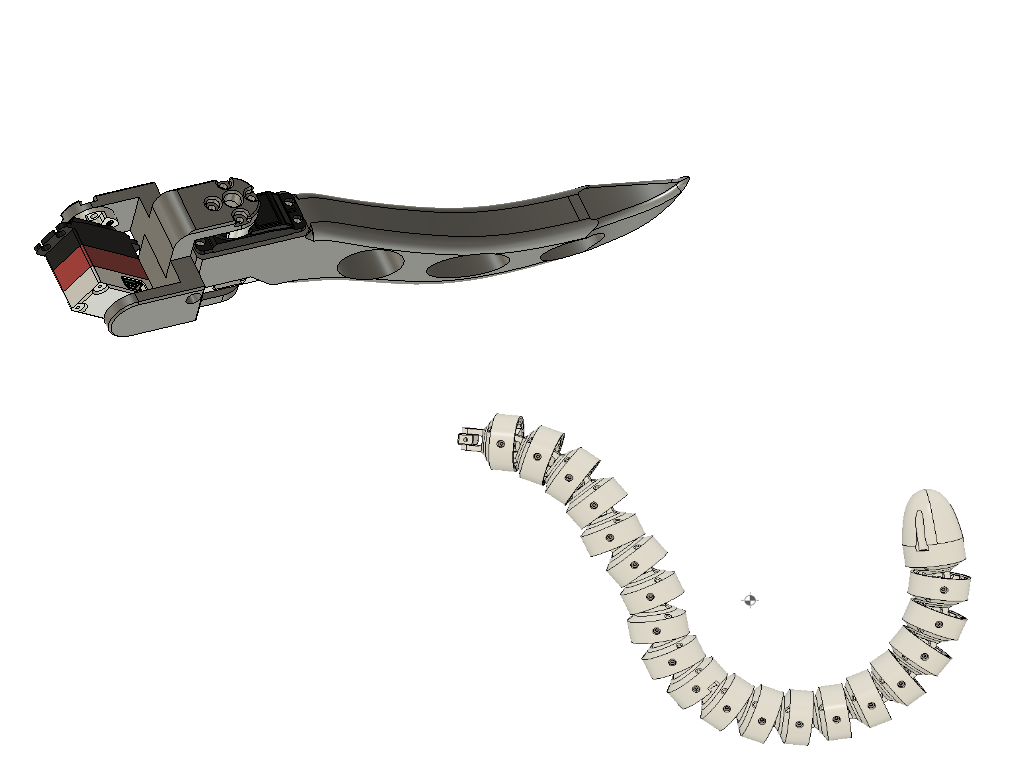
\includegraphics[width=0.7\textwidth]{figures/Tail.png}
                \caption{SmallKat's Solid Tail [Left] vs Continuum Tail [Right]}
                \label{fig:TailComparison}
            \end{figure}
        
        % add info and pictures regarding pla and ninja flex
        
        \paragraph{PLA and NinjaFlex Experimentation} The design for a continuum robot is pretty straight forward. There are a series of disks that are driven by 3 or more wires. Several designs will include springs or means of tension to provide some resistance and stability to the system. These springs will either be placed along the backbone of the tail or in between each disk along the path of the springs. When brainstorming ideas for how we were going to make the tail a thought came to us. By 3D printing the tail out of a firm flexible material we could customize the design and make the assembly process a lot easier. There were several iterations of this design made. The first tail was printed entirely out of NinjaFlex. The design provided the firmness and flexibility we were looking for however the design wasn't suited for bending as much as we needed it to. Additionally NinjaFlex prints much slower than other filaments. As a result we decided to combine our 3D printed idea with other standard designs that we researched a create a design with a single cored backbone. In order to cut down on print time we ended decided to experiment with dual extrusion printing and use two materials to create our tail. The result was several iterations of PLA and NinjaFlex tails that had different sized plates and cores. The final design resulted in a fair amount of success and was actually turned into a fully functional prototype.
        
         \begin{figure}[H]
                \centering
                \includegraphics[width=0.7\textwidth]{figures/DualExtrudedDesigns.jpg}
                \caption{Dual extruded designs}
                \label{fig:DualExtrudedDesigns}
        \end{figure}
            
         \begin{figure}[H]
                \centering
                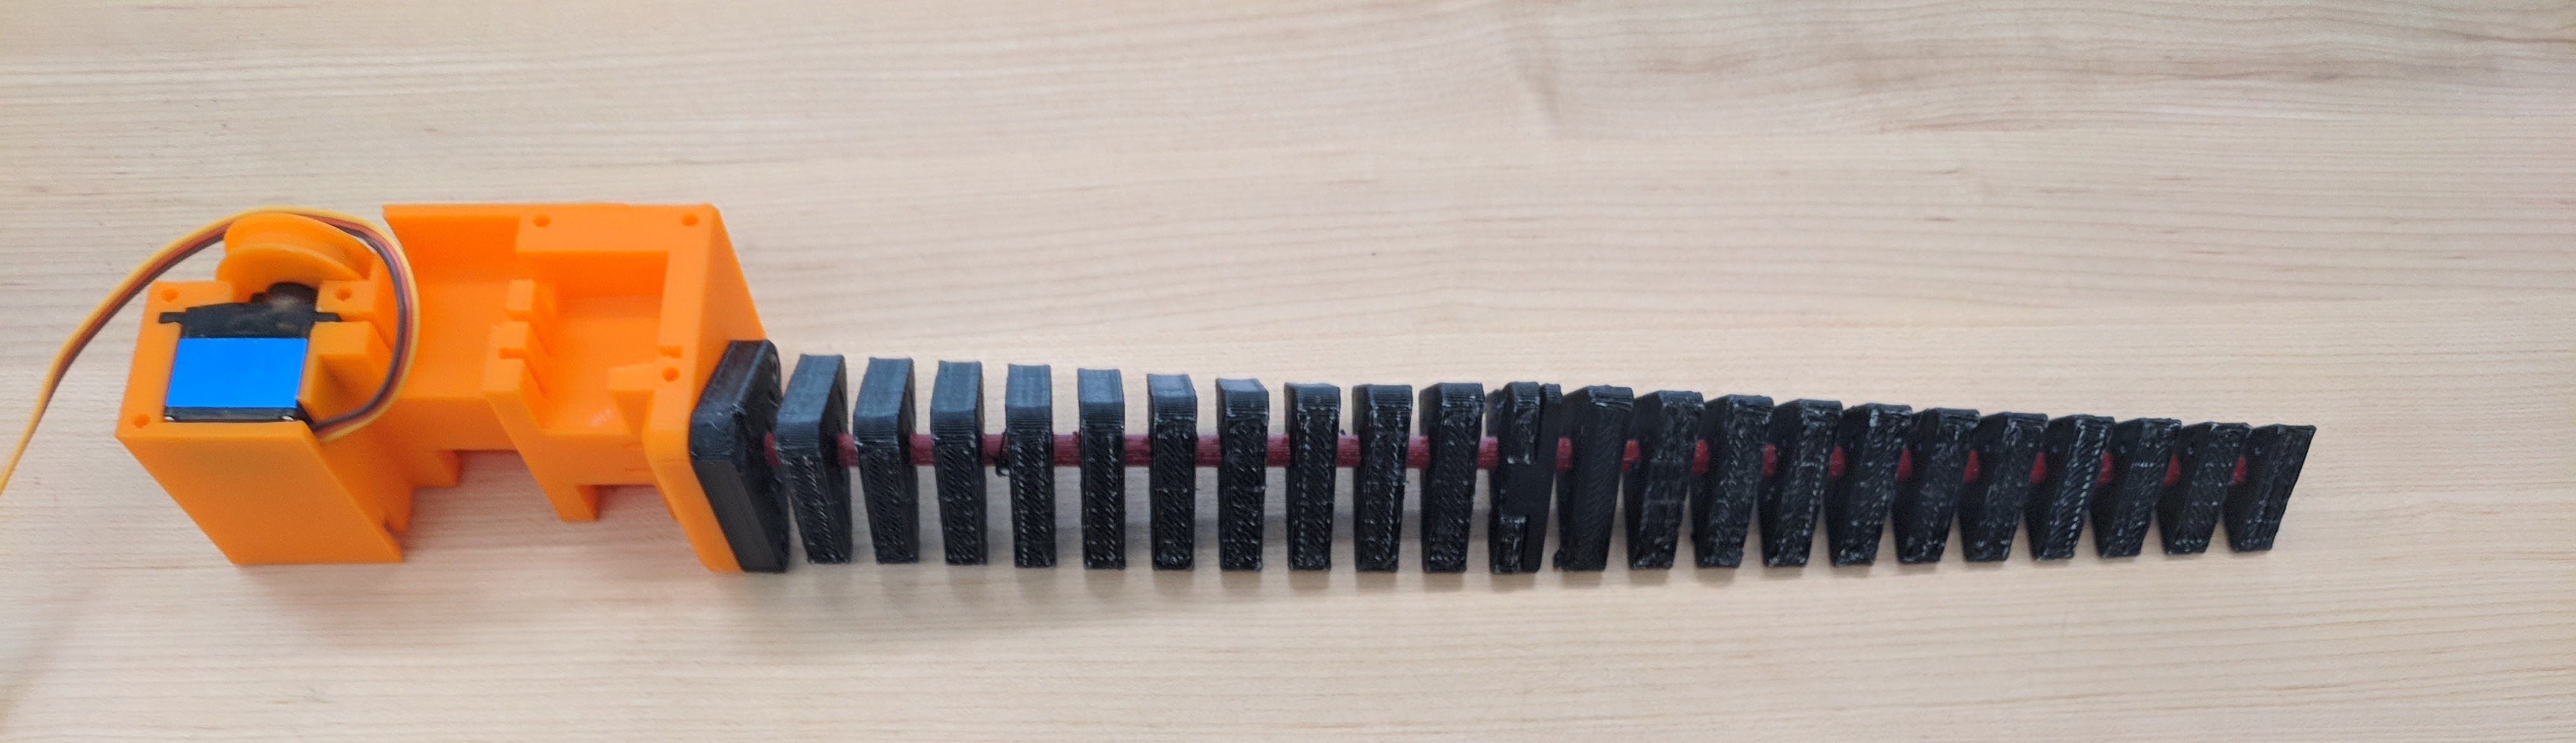
\includegraphics[width=0.7\textwidth]{figures/NinjaFlexTail.jpg}
                \caption{First full prototype of NinjaFlex tail}
                \label{fig:FirstPrototype}
        \end{figure}    
        
         \begin{figure}[H]
                \centering
                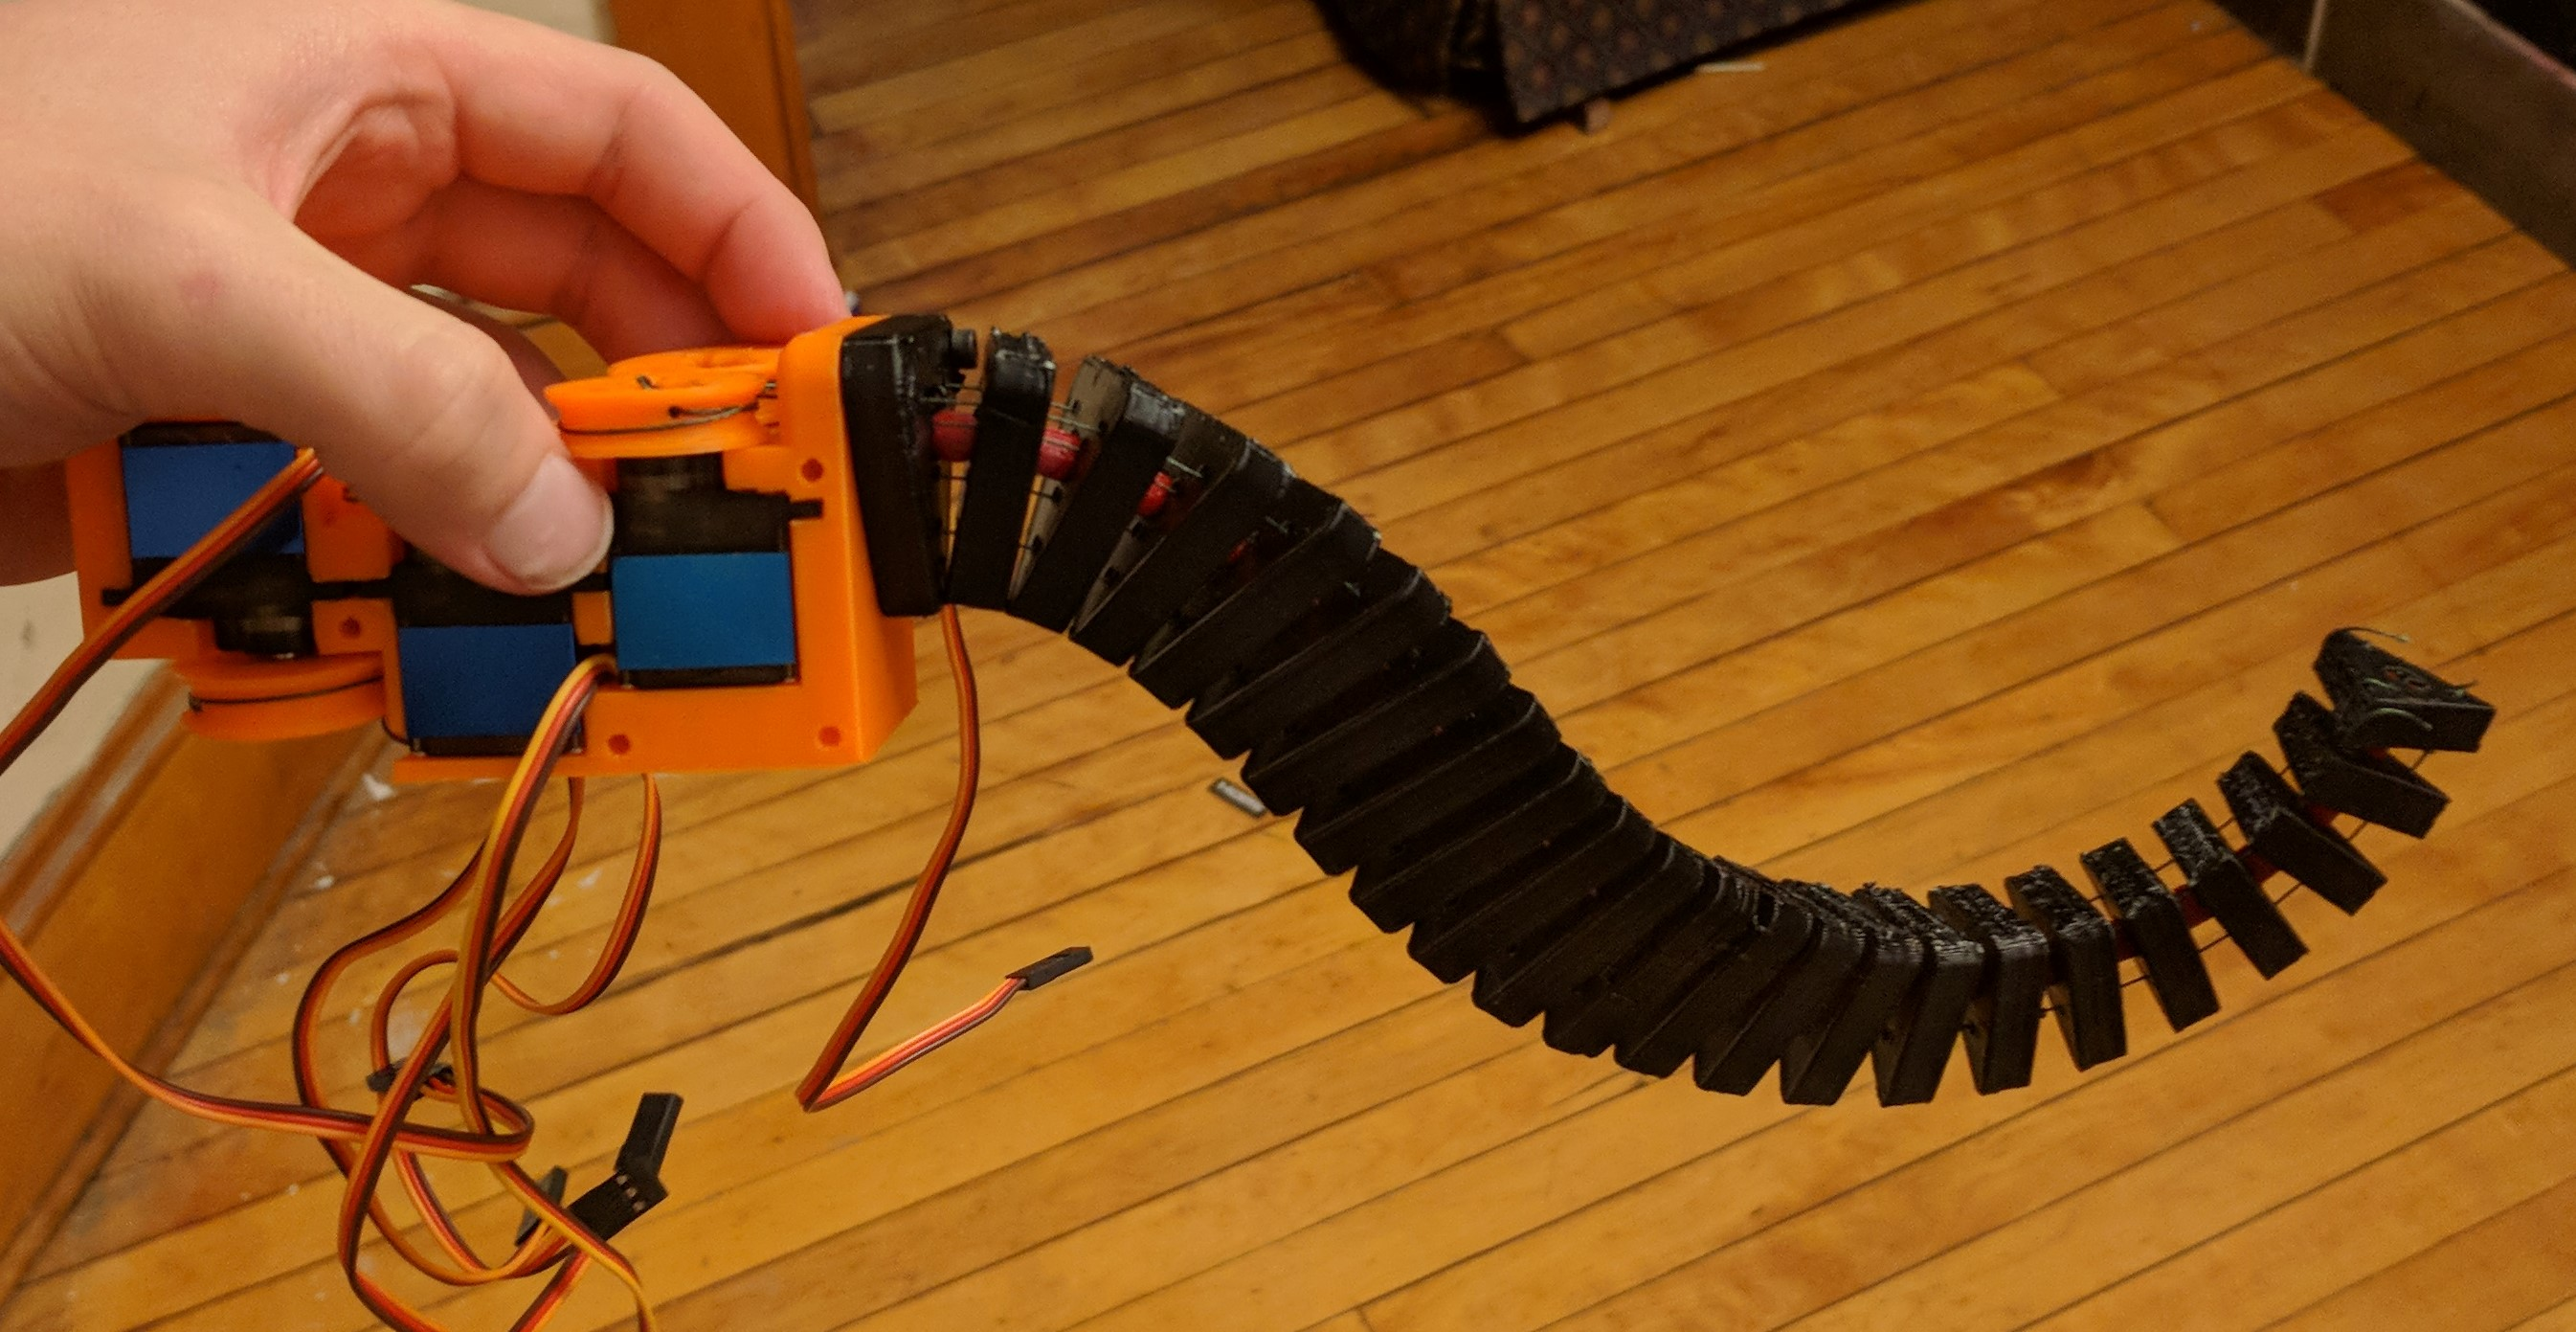
\includegraphics[width=0.7\textwidth]{figures/FirstPrototype1.jpg}
                \caption{Prototype of NinjaFlex tail with strings}
                \label{fig:FirstPrototypewithstrings}
        \end{figure} 
            
         \paragraph{Universal Joint Design} While the dual extruded design surpassed our expectations it didn't quite provide the level of performance we were looking for. In our tests we were able to control the tail and it was flexible enough, however there was to much play in the system. There was nothing preventing the tail from waving widely out of control when bumped or moved. There is a possibility that this could be fixed with several more tests and iterations of the design however we decided to move to a more tried and true design. The next design utilized a universal joint that would allow the system to maintain a little more rigidity than the previous design. Each of the segments would be 3D printed, which also allowed us to change the size if needed and the whole thing was held together with small dowel pins and M2 bolts. The design can be seen below.    
           
        \begin{figure}[H]
                \centering
                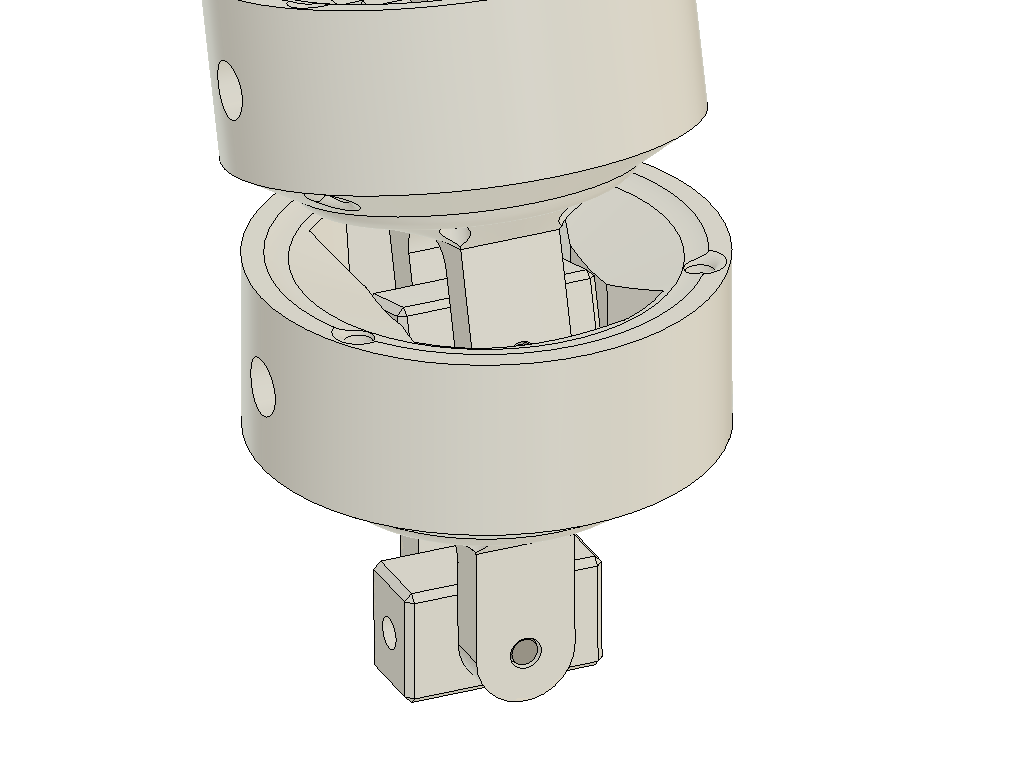
\includegraphics[width=0.5\textwidth]{figures/UniversalJoint.png}
                \caption{Universal Joint}
                \label{fig:UniversalJoint}
        \end{figure}                
            
        \begin{figure}[H]
                \centering
                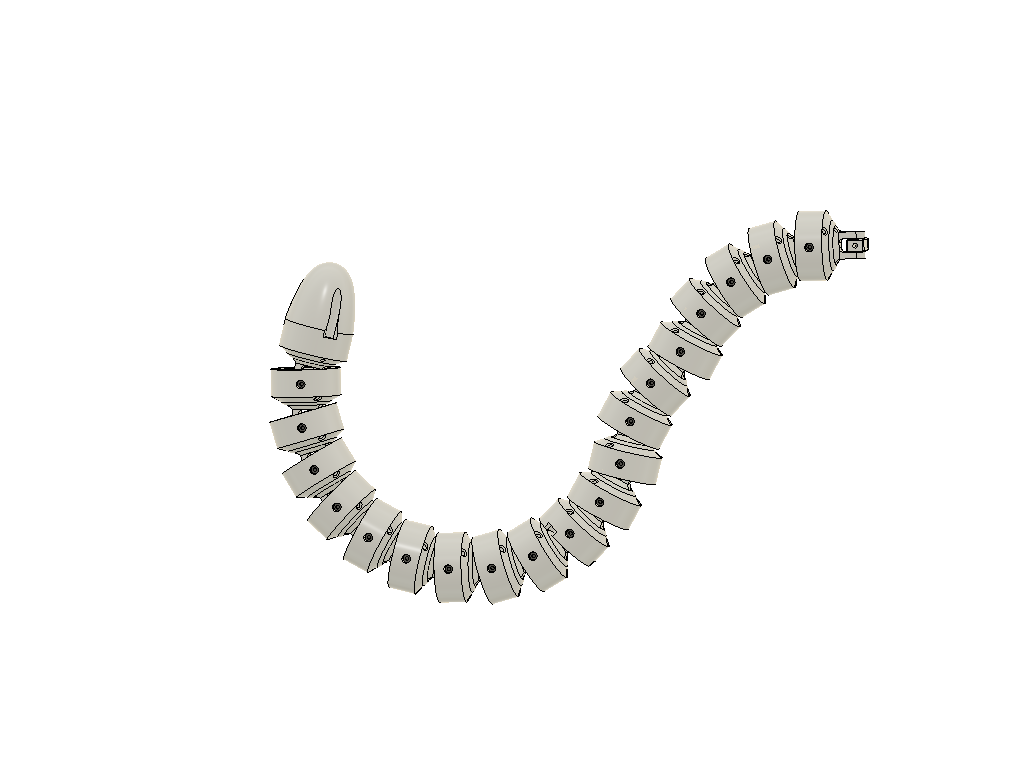
\includegraphics[width=0.5\textwidth]{figures/ContinuumTail.png}
                \caption{Universal Joint Tail}
                \label{fig:UniversalJointTail}
        \end{figure}    
        
        \paragraph{Final tail Design}
        The tail design that ended up on the robot had two segments that could be individually controlled. Each segment was controlled by 2 Maxon motors that would spool the top two strings of the three. The last string was connected to a spring that would a apply constant force to the tail causing it to curl down. The rational behind this was that the tail would only need to move left right or up and these motions could be done with only two motors. Additionally we saved a lot of space by eliminating two motors. The motors had encoders on them which allowed us to track their position. However they were not absolute meaning that once the robot was turned off they would lose their position. To solve this problem a set of limit switches were added in so that the motors could move until they triggered the limit switch and home their position. The final motor setup can be seen below.
        
        \begin{figure}[H]
                \centering
                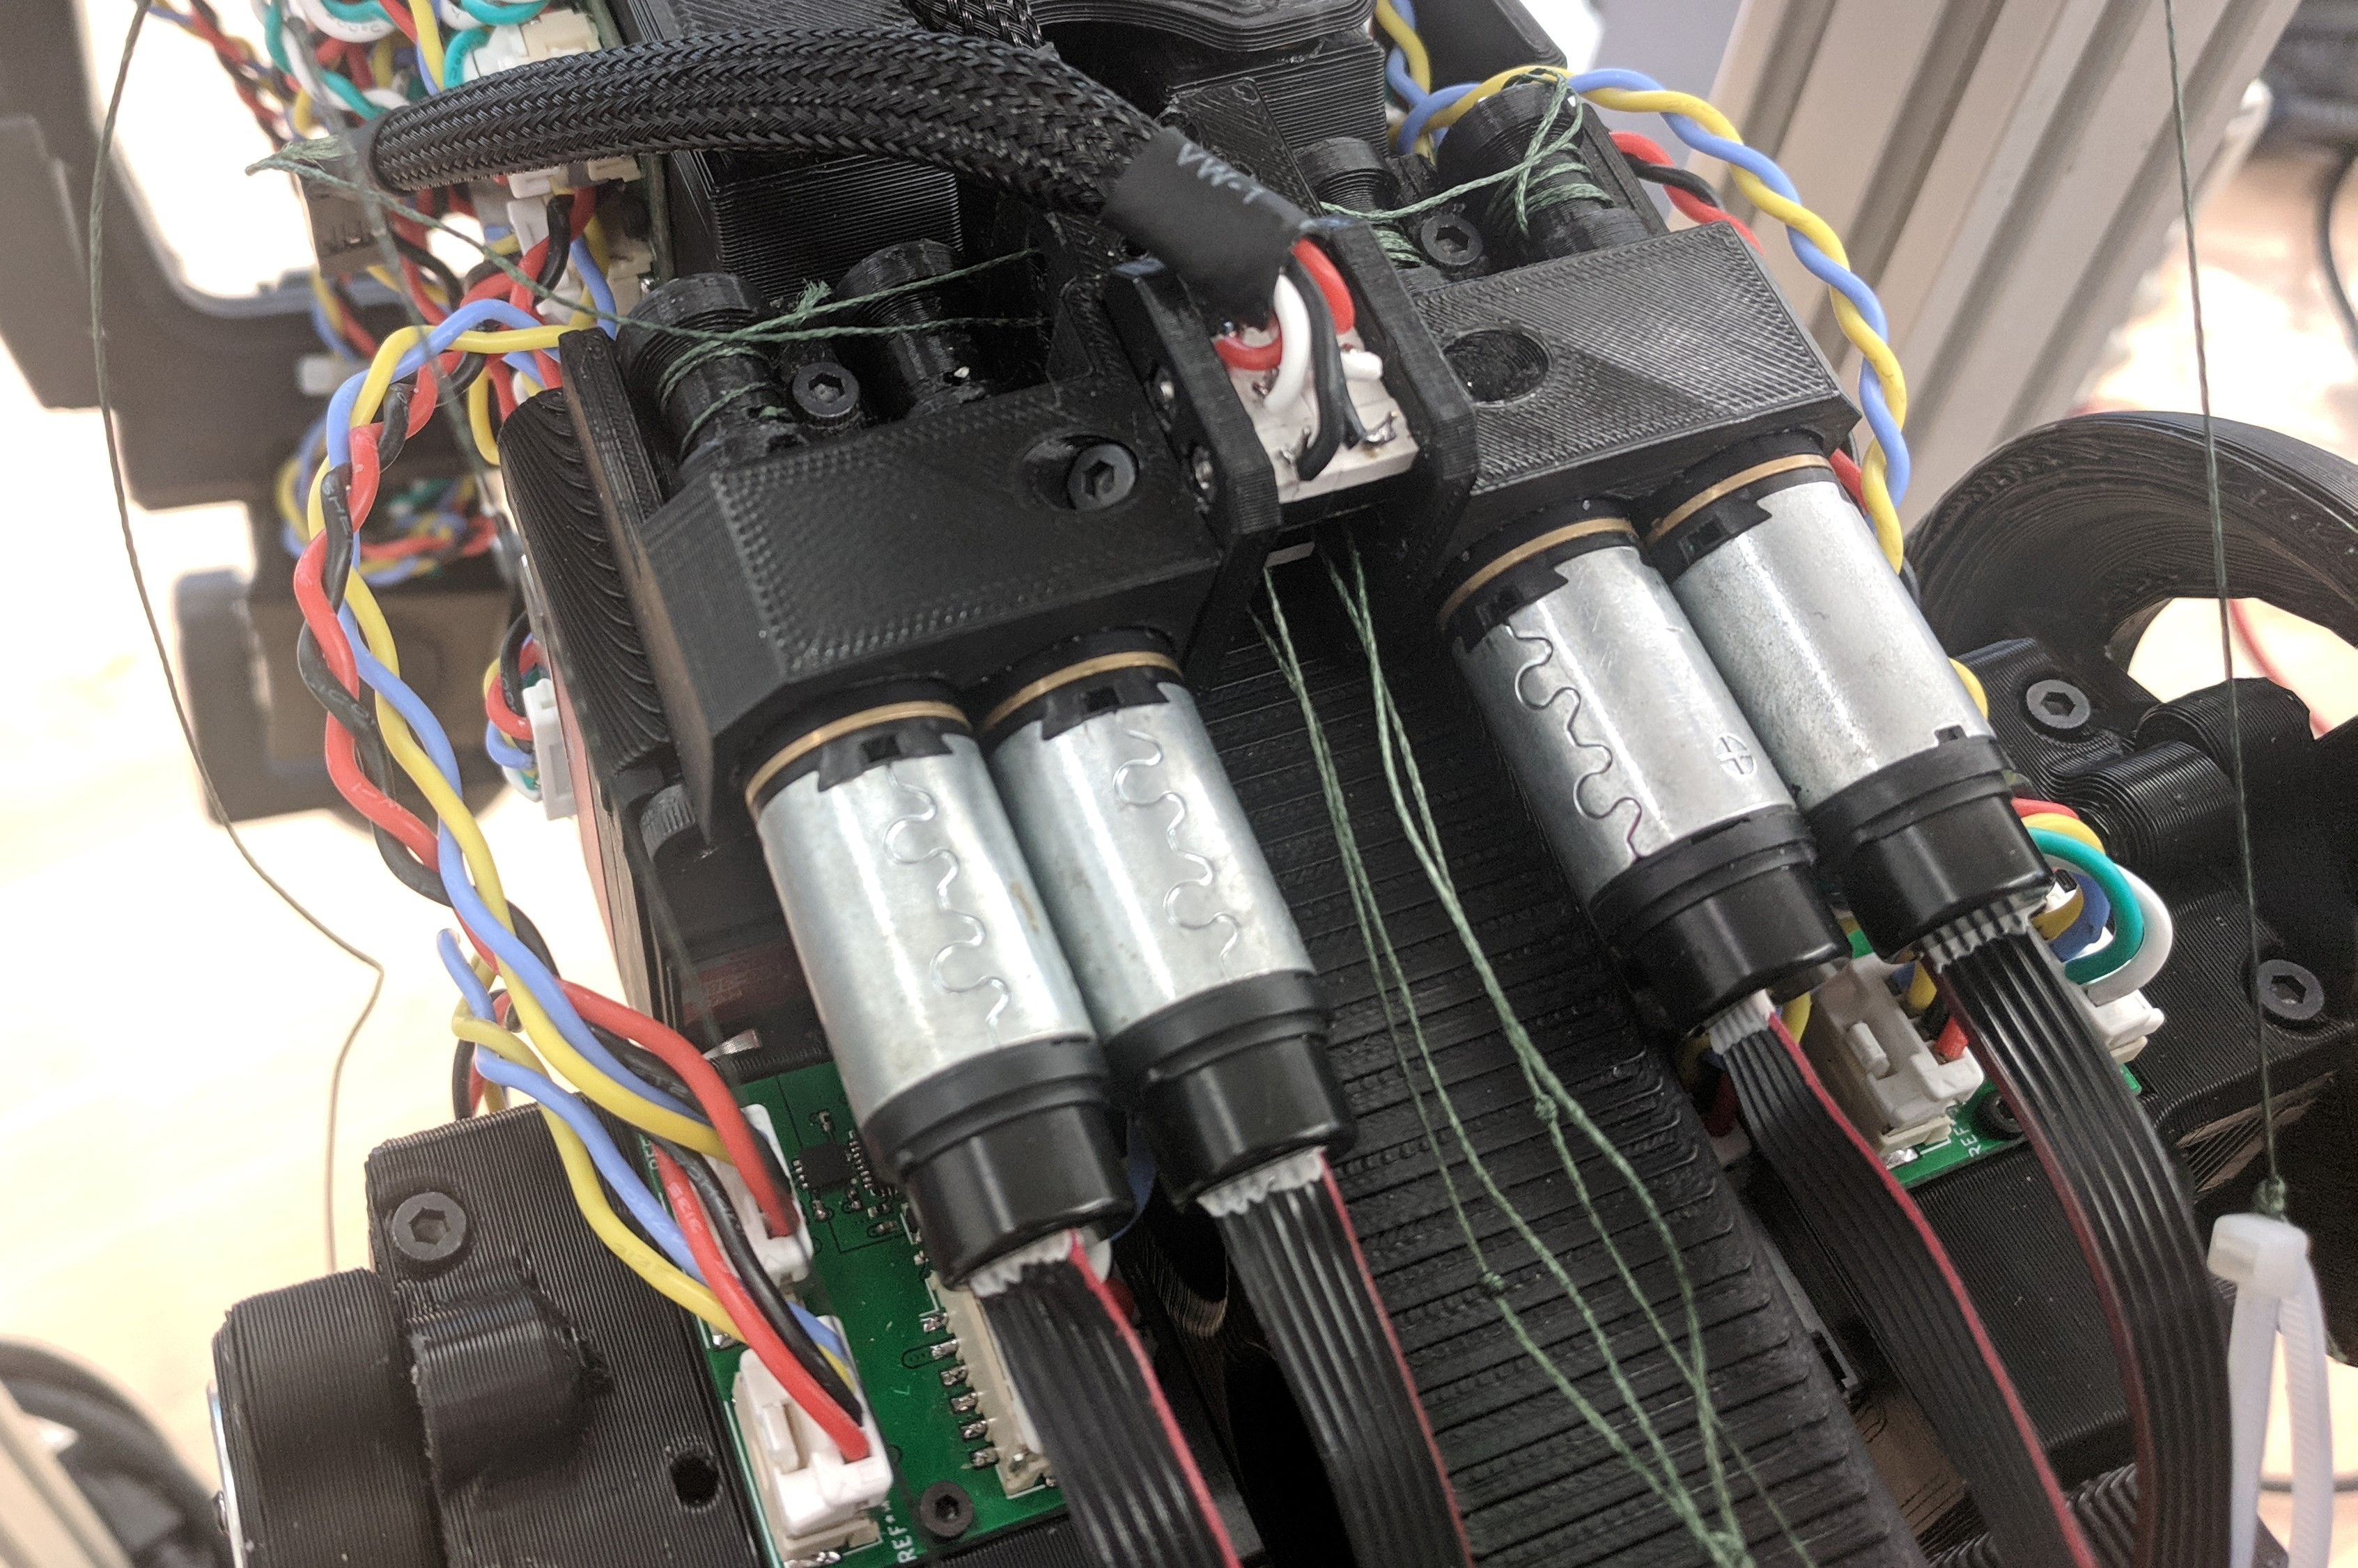
\includegraphics[width=0.5\textwidth]{figures/FinalTailDesign.jpg}
                \caption{Final tail design}
                \label{fig:Finaltaildesgin}
        \end{figure}   
            
        \subsubsection{Design Iterations} 
        
       \paragraph{Sizing SmallKat}
         When deciding the size of SmallKat, we looked into the options currently provided on the market, as well as previous versions (talked about in Section \ref{subsec:SmallKatVersions}). Larger robots like Boston Dynamics' Big Dog and Spot Mini robots were rather large, and would increase the cost of the robot as a whole. When looking at SmallKat V2, we appreciated its "desktop" size, but realized it's small form factor also limited us in our goals. Since deciding on an exact size was difficult, we decided to size our robot based on a standard servo. This would allow users to swap motors with others that better suit their needs without having to redesign the whole robot. In the end, our robot ended up being slightly larger than a standard house cat. While the robot is still small and relatively nimble, it also has the capability to have advanced sensors, like a 3D Real Sense camera, and to traverse paths that the smaller SmallKats couldn't, like stairs. 
        
        \paragraph{First Design}
        The first leg design of the SmallKat MQP design was just a rough draft without specifications of motor torque or how big the leg could be. The design experimented with a design for the elastic spring system that used an embedded spring instead of the bungee cords we had tested with because it was designed before those tests.However, there was some difficulty embedding a big enough spring. Because there weren't many technical specifications to go off this iteration focused on aesthetics and making a design that could be printed. 
        
       \begin{figure}[H]
          \centering
          \begin{minipage}[b]{0.4\textwidth}
            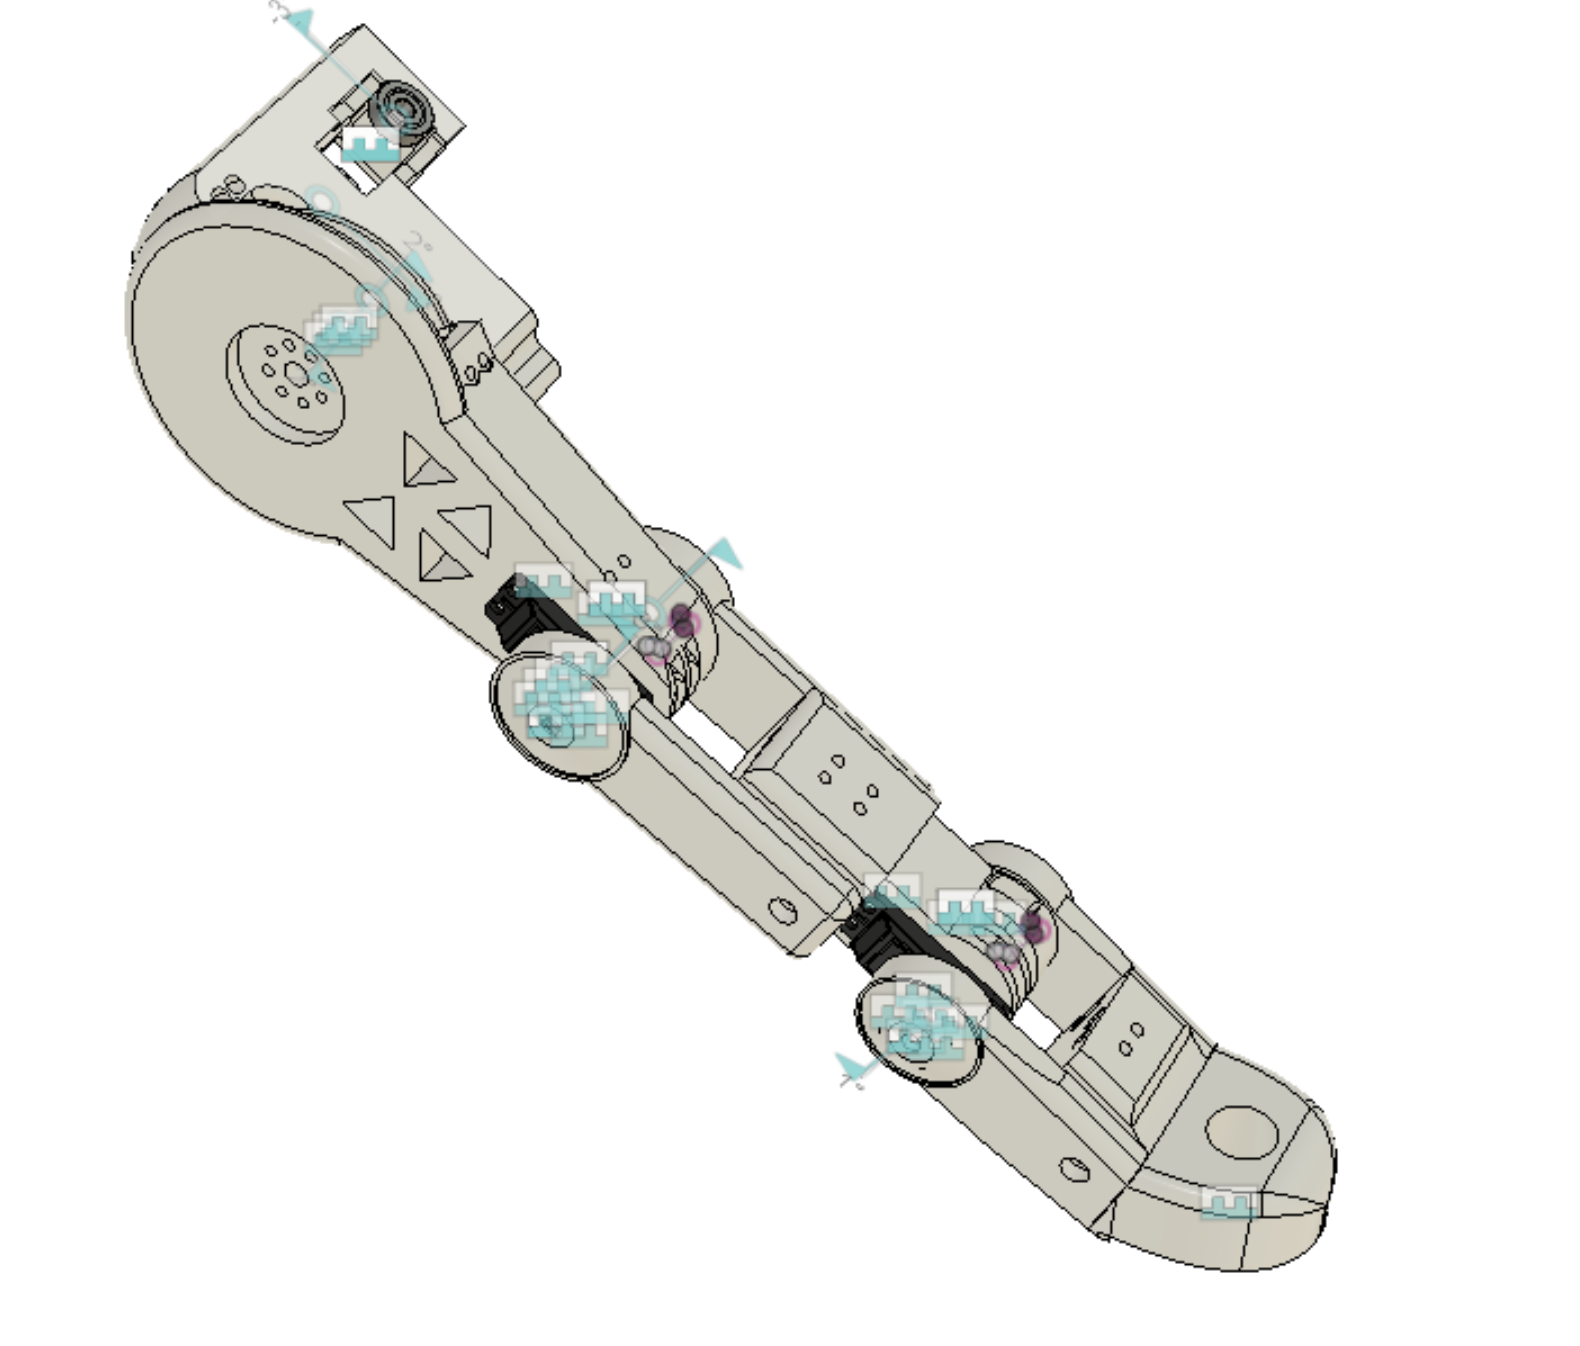
\includegraphics[width=\textwidth]{figures/PrototypeLeg1.PNG}
            \caption{First Prototype Leg}
            \label{fig:FirstPrototypeLeg}
          \end{minipage}
          \hfill
          \begin{minipage}[b]{0.4\textwidth}
            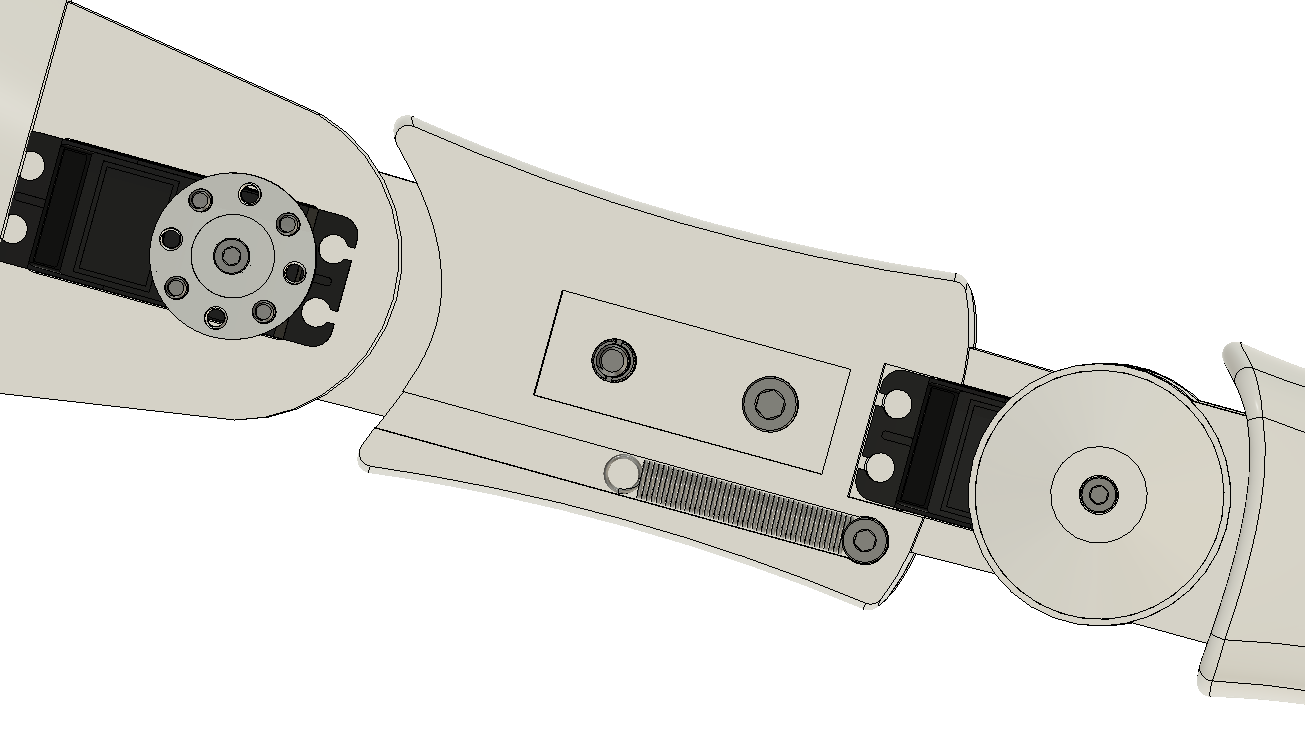
\includegraphics[width=\textwidth]{figures/IntegratedSpring.png}
            \caption{Integrated Spring Design}
            \label{fig:IntegratedSpringDesign}
          \end{minipage}
        \end{figure}
        
        \paragraph{Second Design}
        The second design was also made to be the largest possible leg with the motor torques and the spring assist. We were able to do this by incorporating the bungee cords that were tested earlier in the project and the motor torque data that we had collected. In order to attache the bungee cords the were stuck through holes in each limb and then set screwed into place. Channels then guided them around the leg allowing them stretch when the leg rotated. We ended up printing and assembling this design however, it turned out to be very large. After further deliberation it was decided that if we could make the robot smaller and not have to need a elastic spring system it would a lot easier to control in the control system. 
        
         \begin{figure}[H]
                \centering
                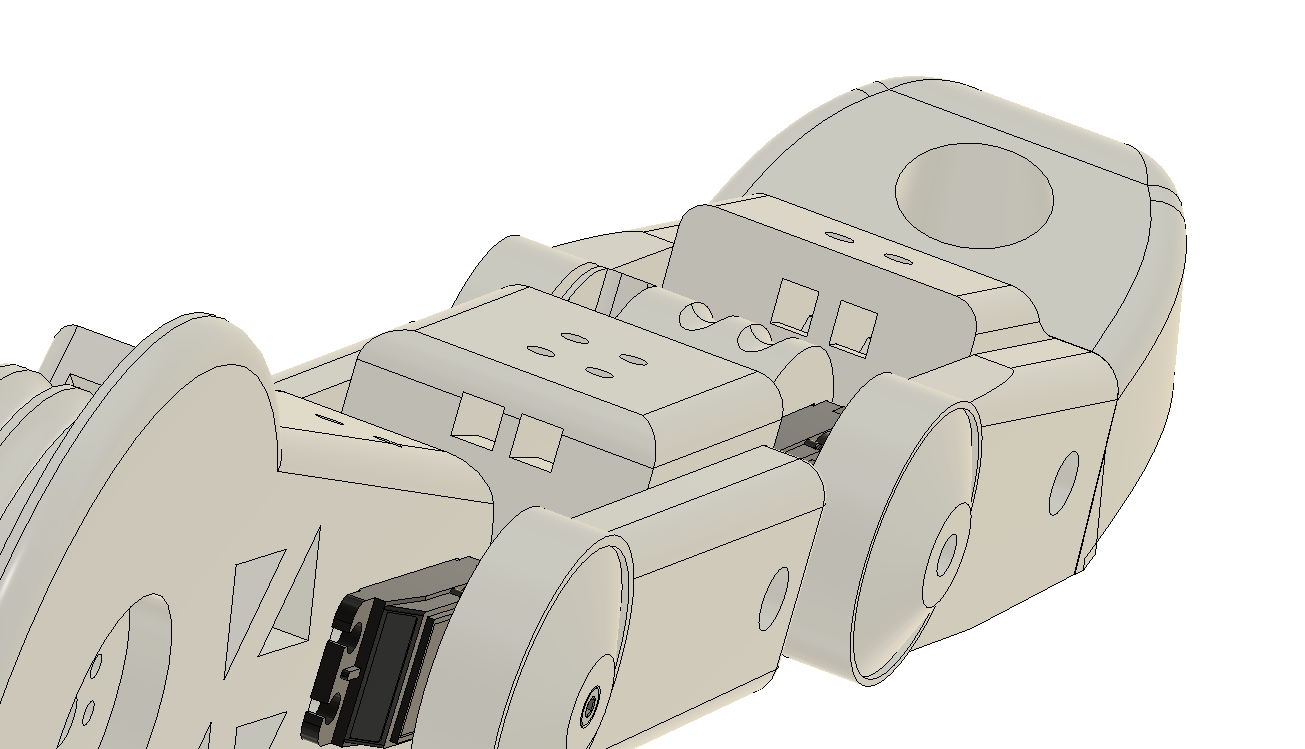
\includegraphics[width=0.5\textwidth]{figures/Prototype2.png}
                \caption{Second Prototype Leg}
                \label{fig:SecondPrototypeLeg}
        \end{figure}                
            
        \begin{figure}[H]
                \centering
                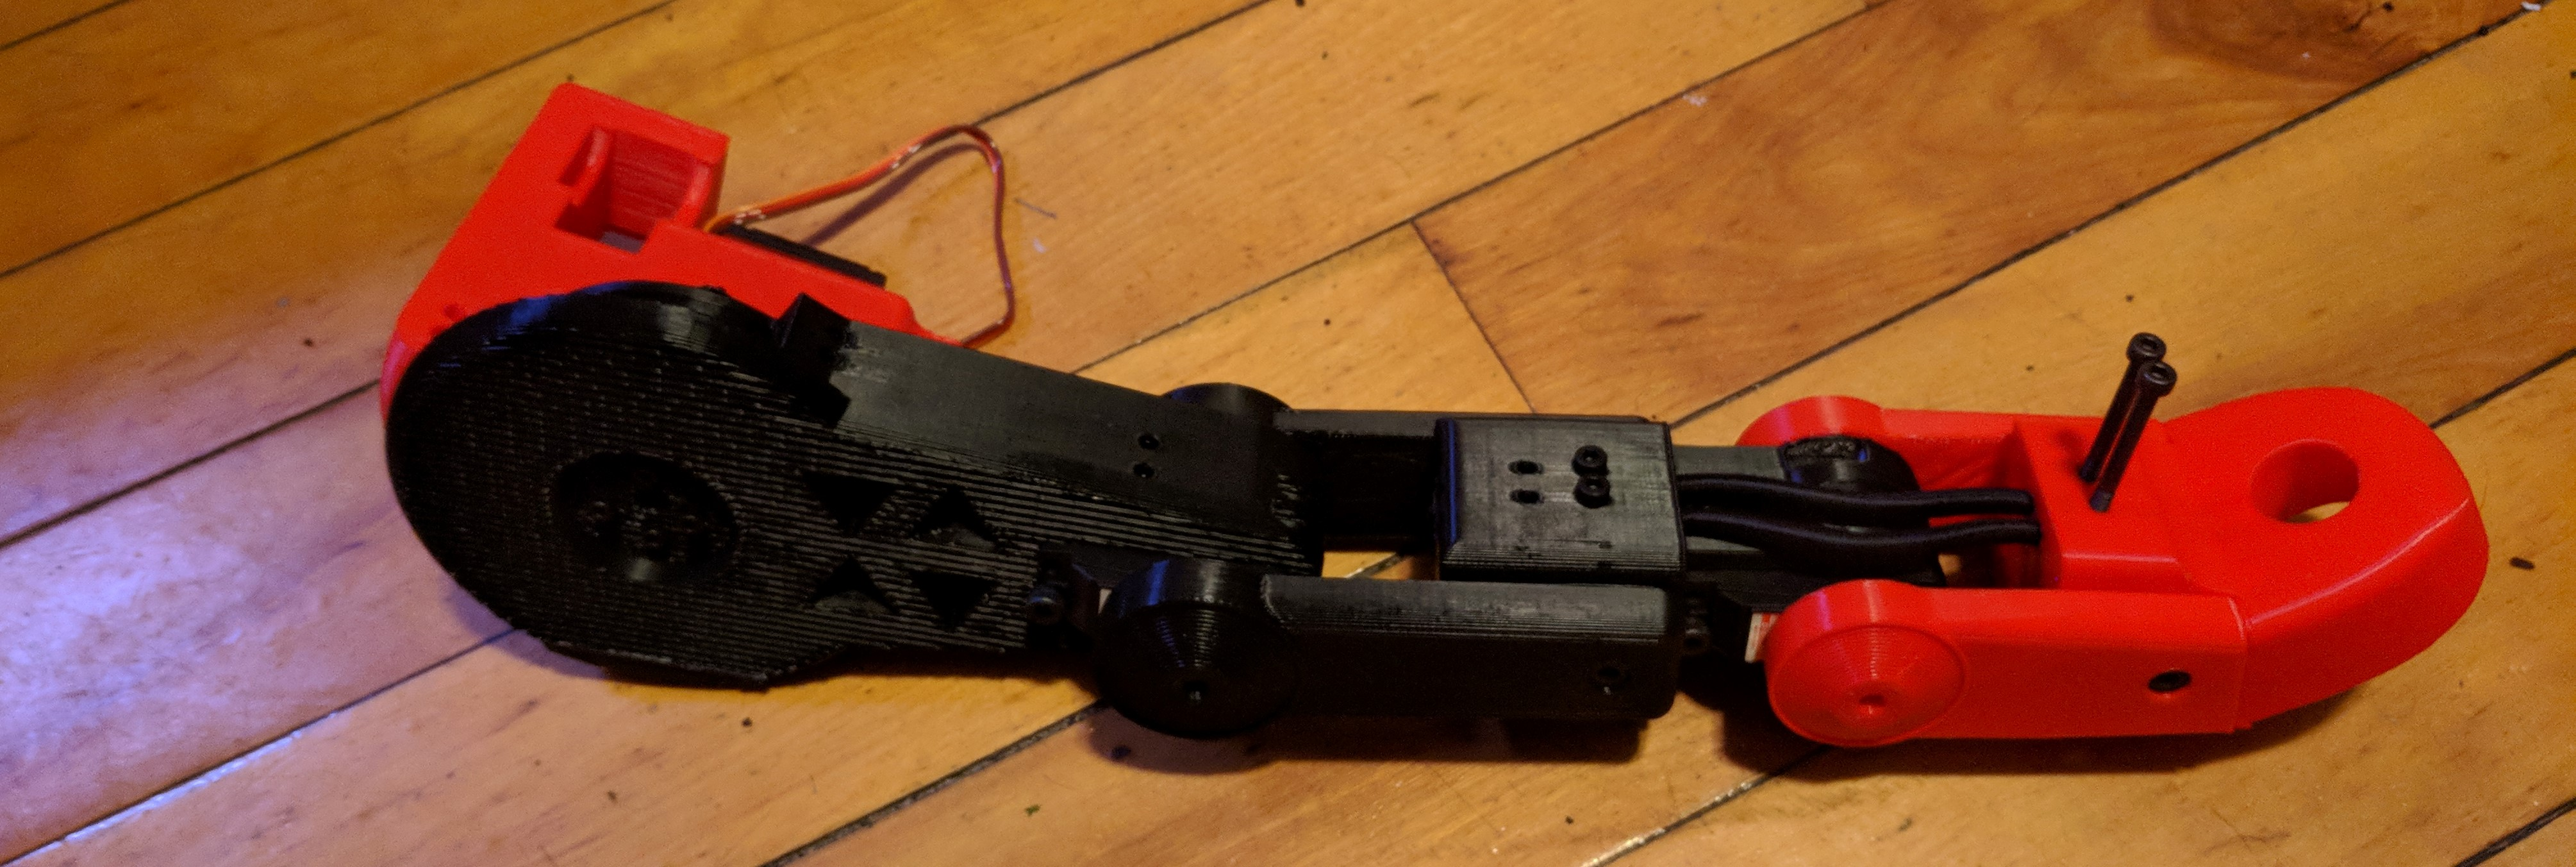
\includegraphics[width=0.5\textwidth]{figures/prototype2printed.jpg}
                \caption{Second Prototype Leg Printed}
                \label{fig:SecondPrototypeLegPrinted}
        \end{figure}    
        
        \paragraph{Third and Fourth Iterations}
        The third design experimented with a new way of mounting servos. The two designs before this had the servos in the middle of the leg. However this design has the support coming from the opposite side of the servo horn and allows for the servo to stick out. This design was the first to be iterated with a mock up of the full body. It wasn't a full mock up but the other components were placed in to give a feeling for size and shape. It was determined that in its current configuration the servos on the inside would interfere too much with each other and cause the legs to not be able to move in all the way. As a result the fourth design was modified to have the servos stick out on the outside. This design was the first to be completely printed. The servos were turned to face outwards allowing for mobility on the inside and the legs shorted from previous designs so that it could stand under its own weight without the need of elastics. The overall design was very wide and a bit heavy. Many of the 3d printed parts were over engineered and didn’t need to be as thick as they were. 
        
         \begin{figure}[H]
                \centering
                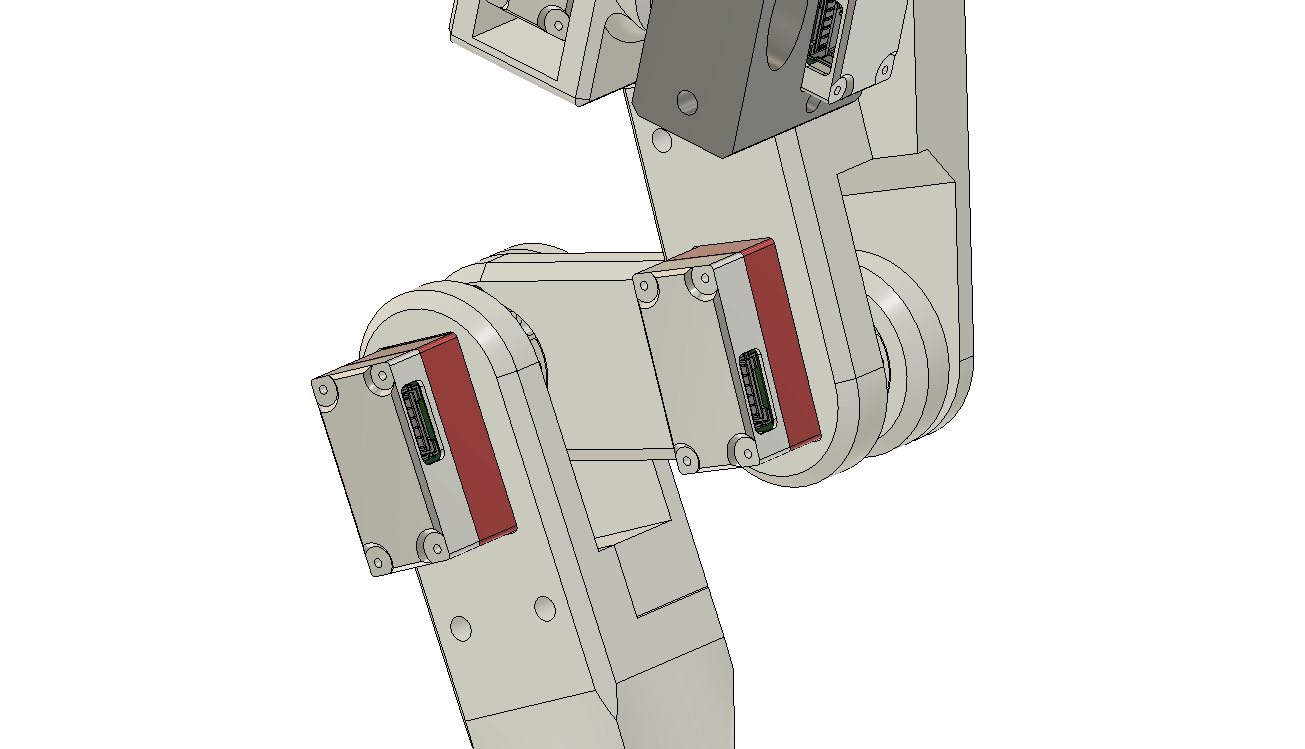
\includegraphics[width=0.5\textwidth]{figures/Prototype3side.png}
                \caption{Side view of third design}
                \label{fig:SideviewPrototype3}
        \end{figure}                
            
        \begin{figure}[H]
                \centering
                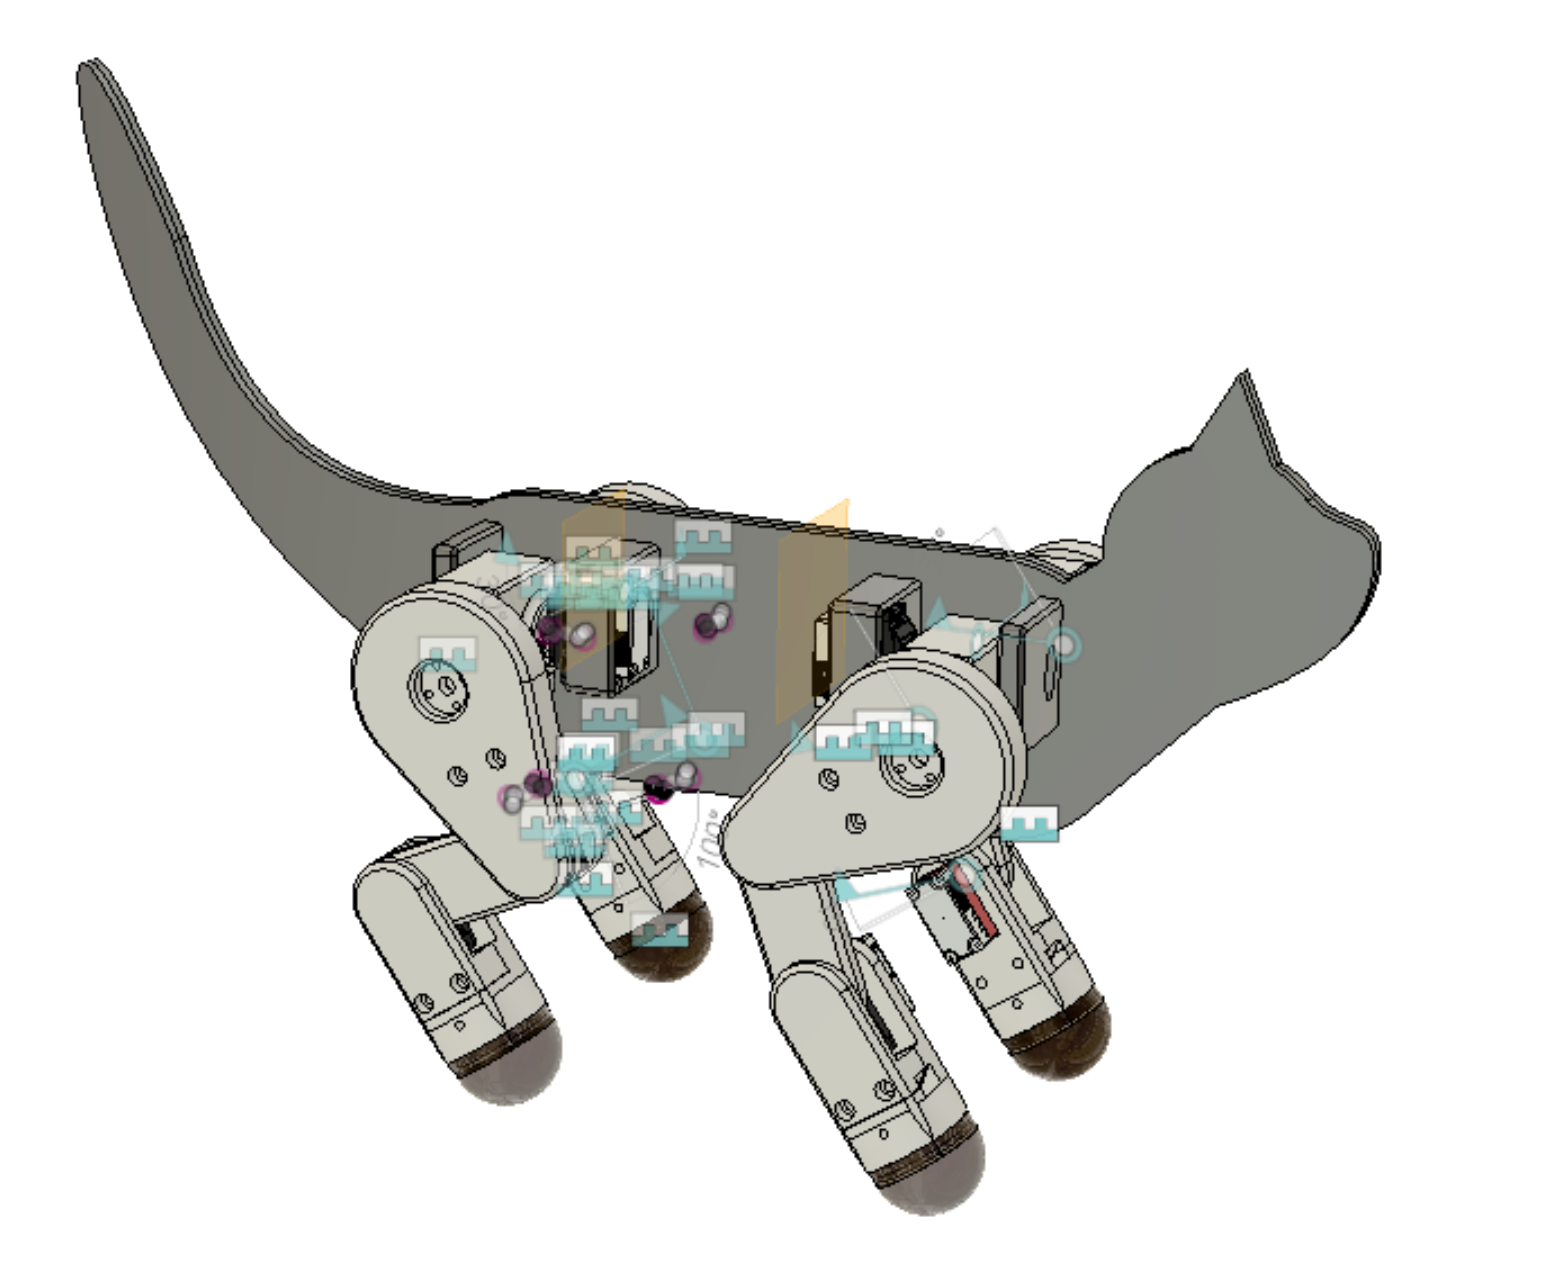
\includegraphics[width=0.5\textwidth]{figures/Prototype3outline.PNG}
                \caption{Prototype 3 with body outline}
                \label{fig:BodyOutlinePrototype3}
        \end{figure}  

          \begin{figure}[H]
                \centering
                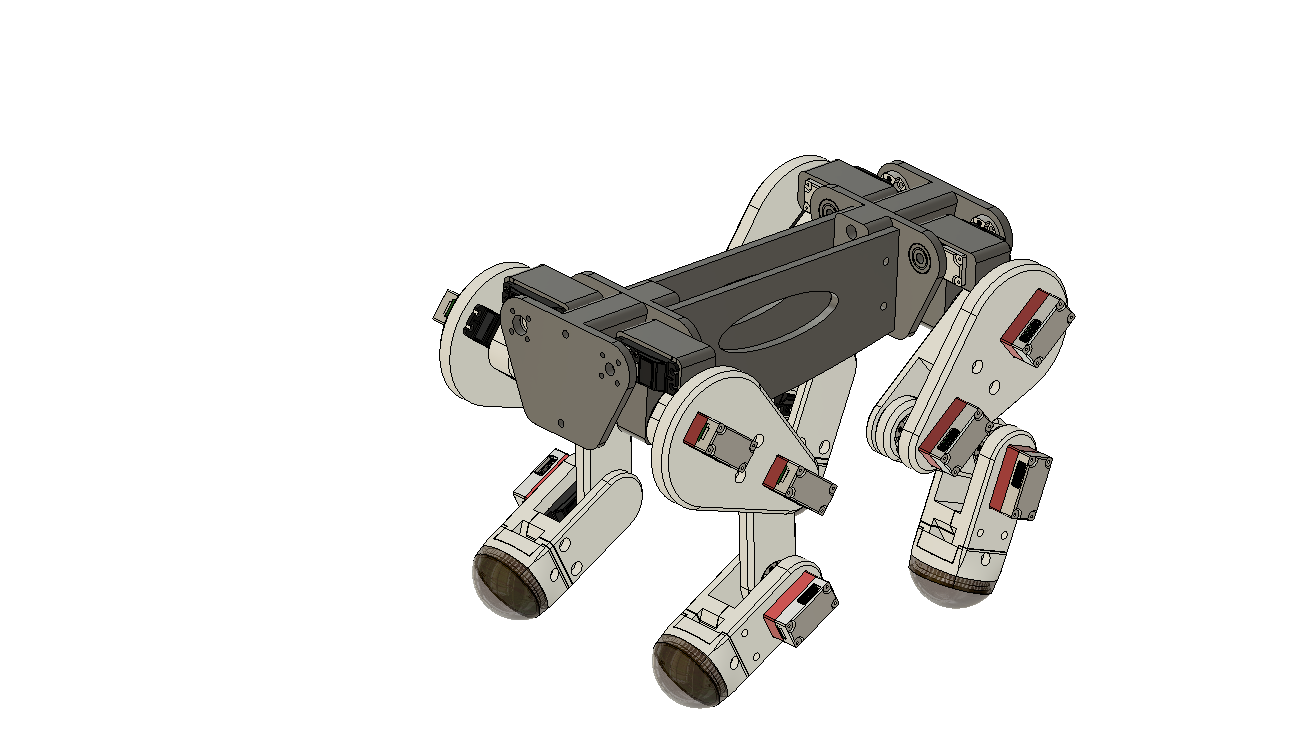
\includegraphics[width=0.5\textwidth]{figures/Prototype4Full.png}
                \caption{Full CAD Model of Prototype 4}
                \label{fig:Prototype4}
        \end{figure}                
            
        \begin{figure}[H]
                \centering
                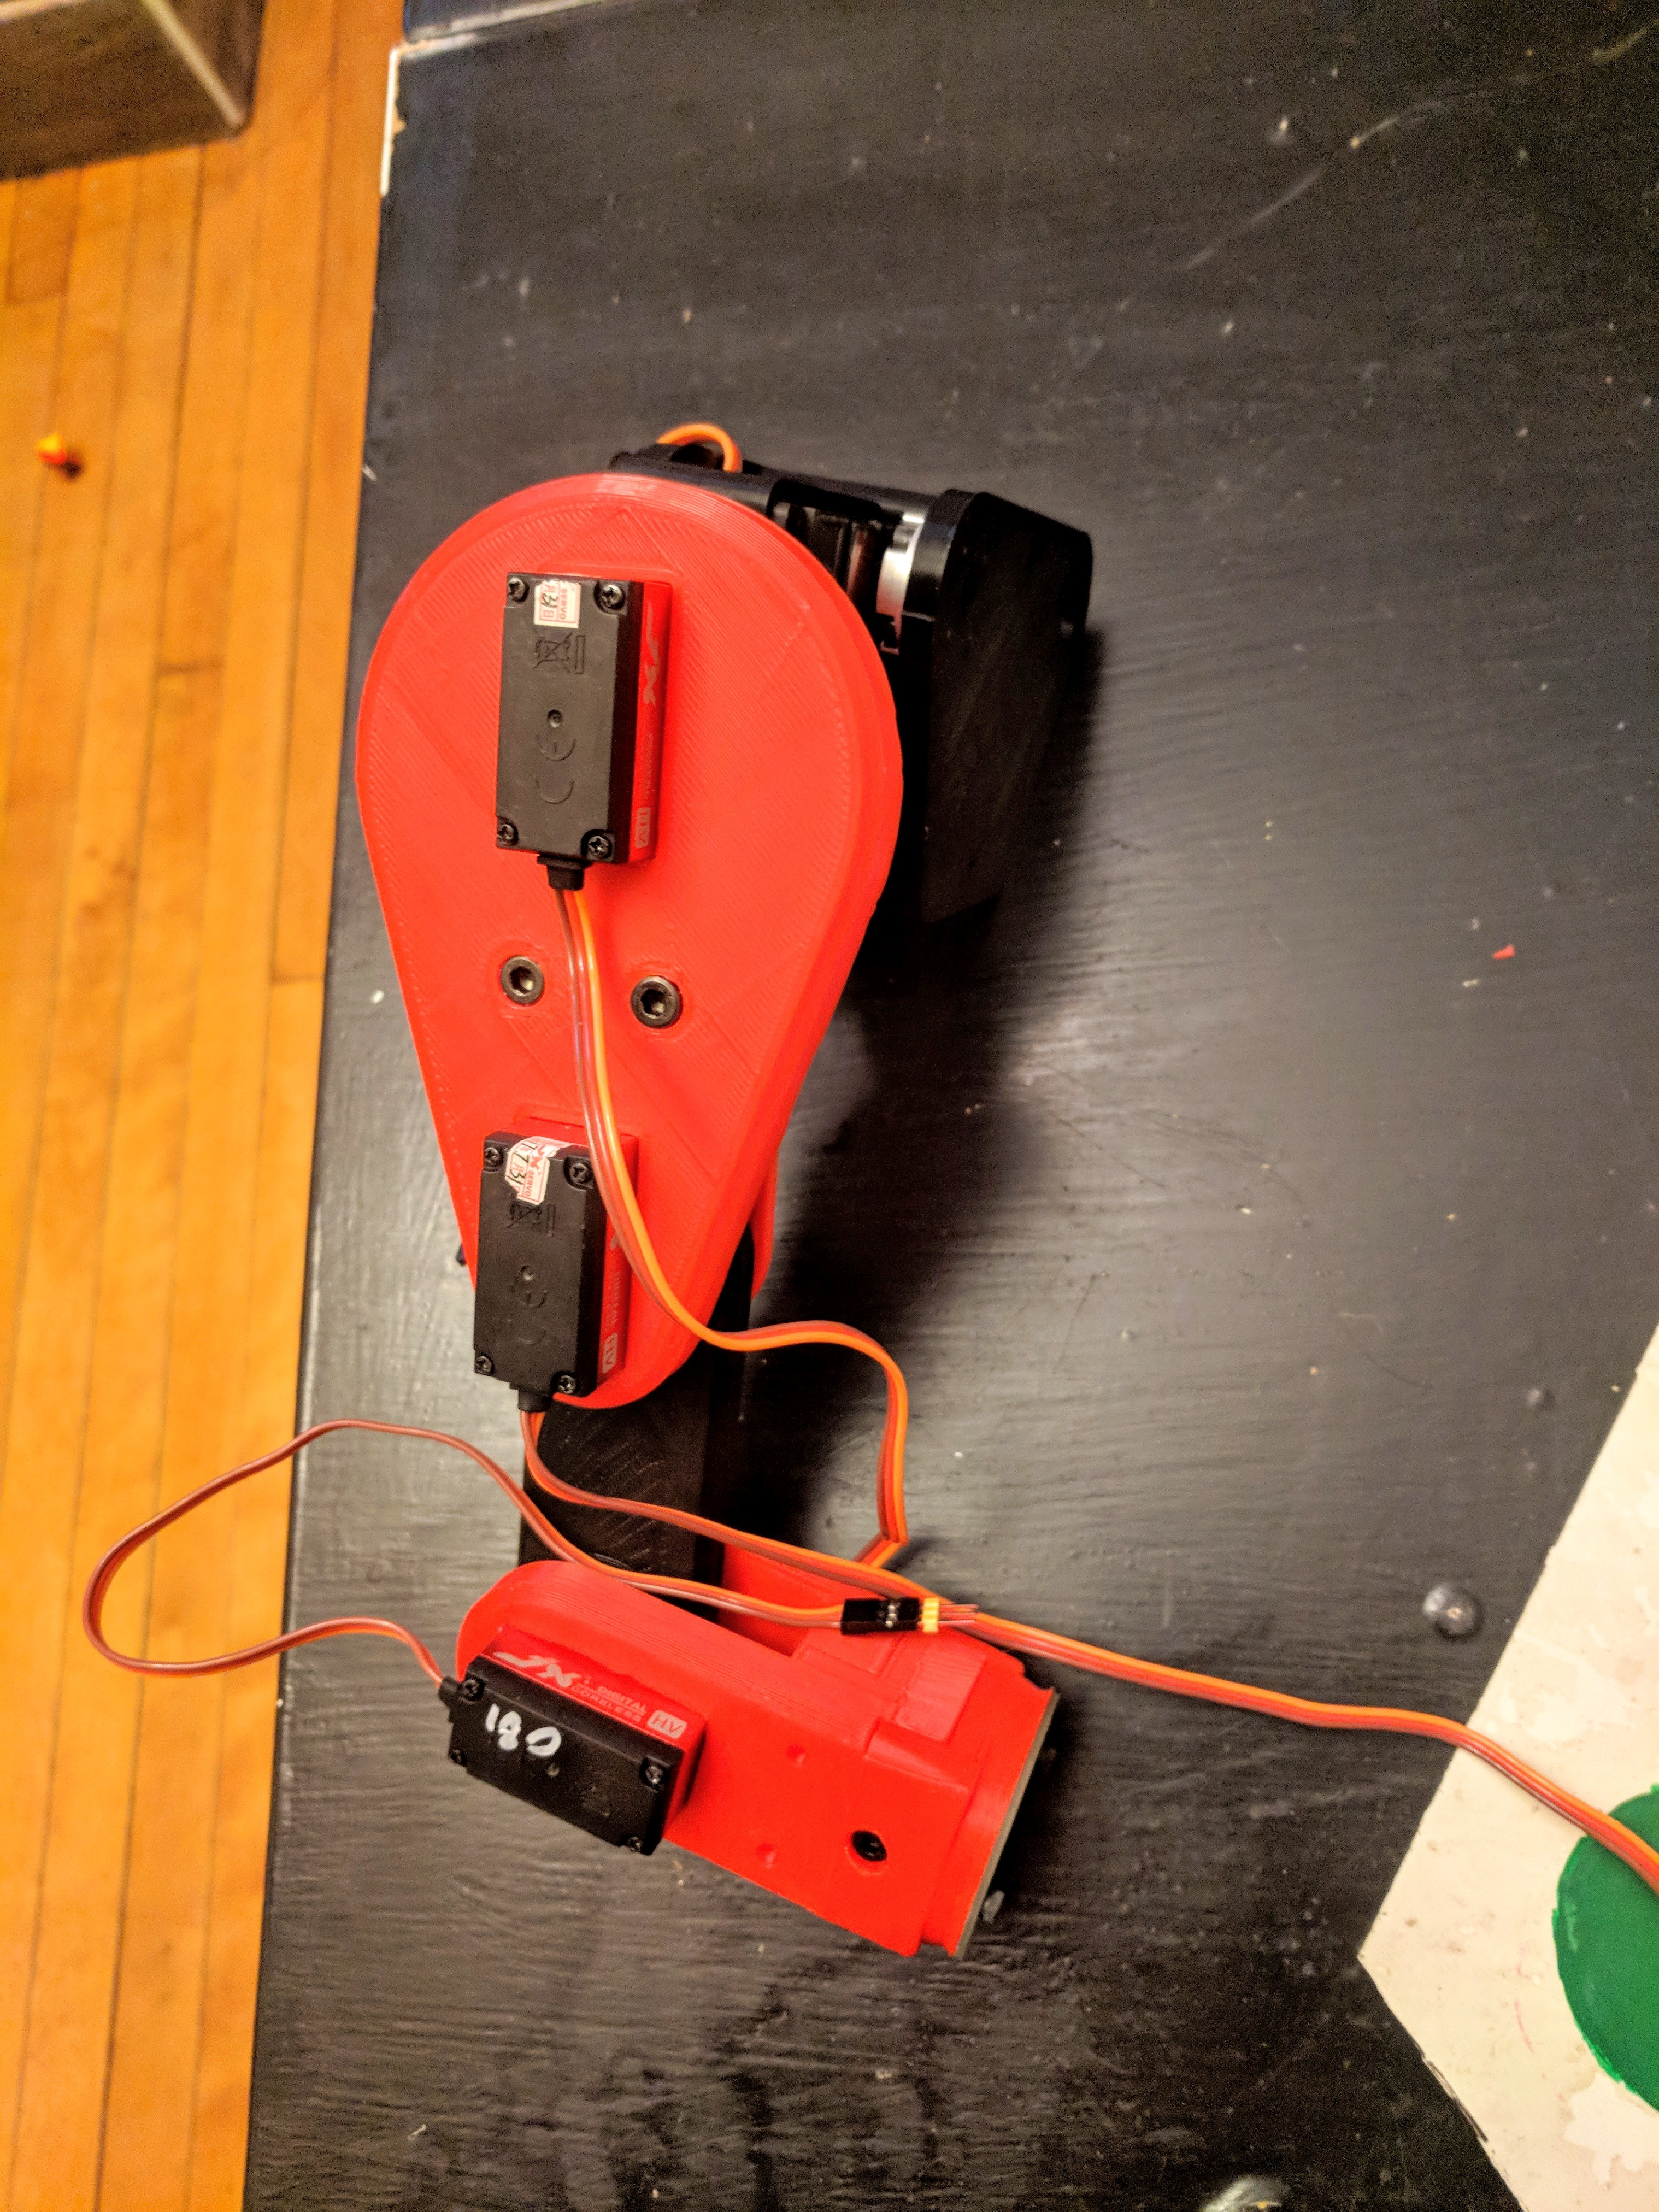
\includegraphics[width=0.5\textwidth]{figures/Prototype4Printed.jpg}
                \caption{Printed Version of Prototype 4}
                \label{fig:Prototype4Printed}
        \end{figure}  
        
        \paragraph{The Conceptual Fifth Design}
        This design was an idea that played off some of the same design feature as the previous design, mainly the fact that the servos were placed on the outside to allow for more mobility and thinner legs. The mid-leg was designed to be machined out of aluminum with the intention of it being much smaller and lighter than previous designs. The top shoulder joint was made significantly smaller than previous designs. The concept was never finished as the supports for the top leg were never added and the legs were still wider than desired. It did however provide some insight into the final design.
         
        \begin{figure}[H]
                \centering
                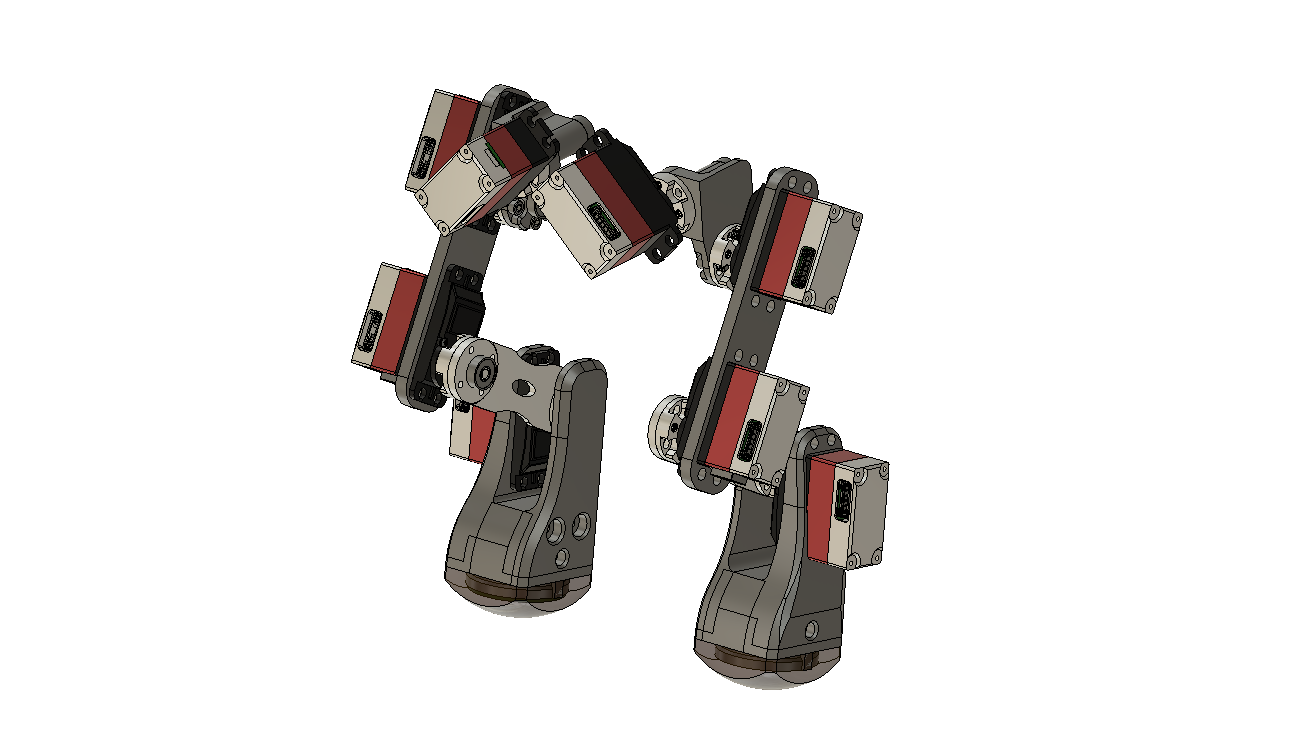
\includegraphics[width=0.5\textwidth]{figures/Prototype5.png}
                \caption{Prototype Design 5}
                \label{fig:Prototype5}
        \end{figure} 
         
        \paragraph{First Full Design}
        After all the revisions and designs, we took everything we had learned and created the first full design of the SmallKat MQP project. The leg design was reverted back to having the servos in line with the legs. By simplifying and reducing the size of the 3d printed part of the legs we were able to keep the size of the hips to a reasonable size relative to the rest of the body. The body itself was designed in two parts for the front and back hips where the legs connected. The tail was a static design with 2 degrees of freedom as the continuum tail had not yet been finished. The head was the same model that had been used for the smaller previous versions of SmallKat except that it was scaled up inside. The neck of this design was given 3 degrees of freedom. The hope was to allow for more movement and give the cat a more natural feel. However it became to complicated and the neck was reduced back to 2 degrees of freedom in the final version. The center of the body held the custom battery back that was made for the robot. This utilized a trap door on the underbelly of the cat that allowed the user to remove the battery when needed. This design was fully printed and assembled to allow us to see size and connections. Below are some pictures of the fully completed prototype.
        
        
         
        \begin{figure}[H]
                \centering
                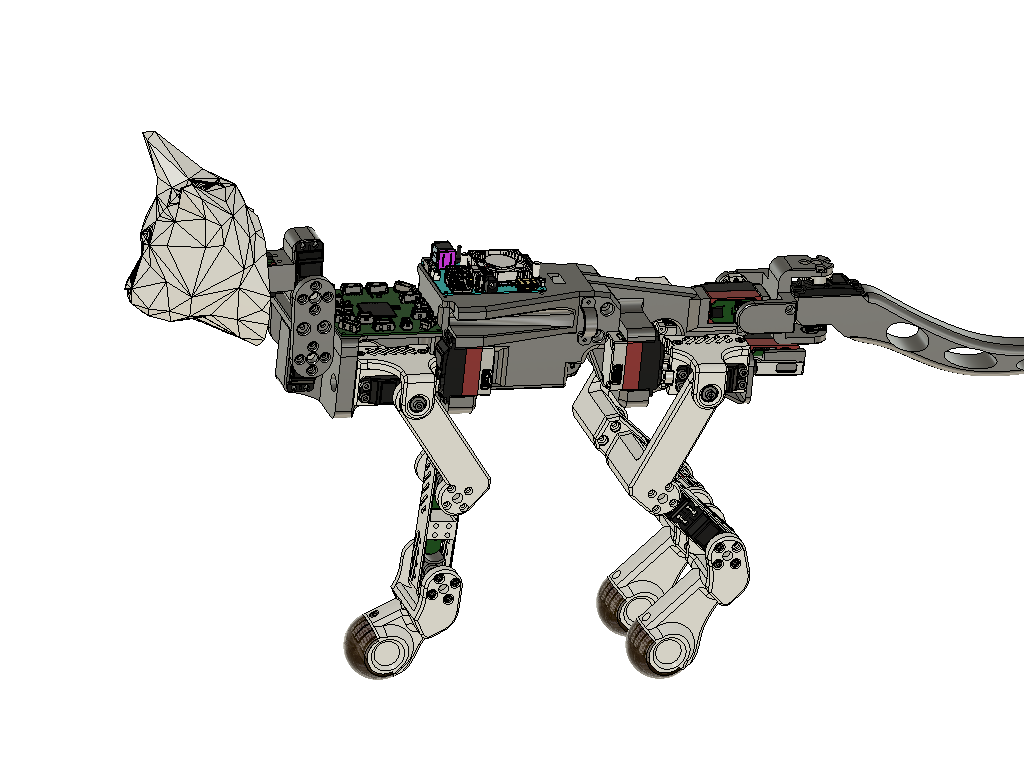
\includegraphics[width=0.5\textwidth]{figures/Prototype6CAD.png}
                \caption{CAD of Prototype 6}
                \label{fig:Prototype6CAD}
        \end{figure} 
        
        \begin{figure}[H]
                \centering
                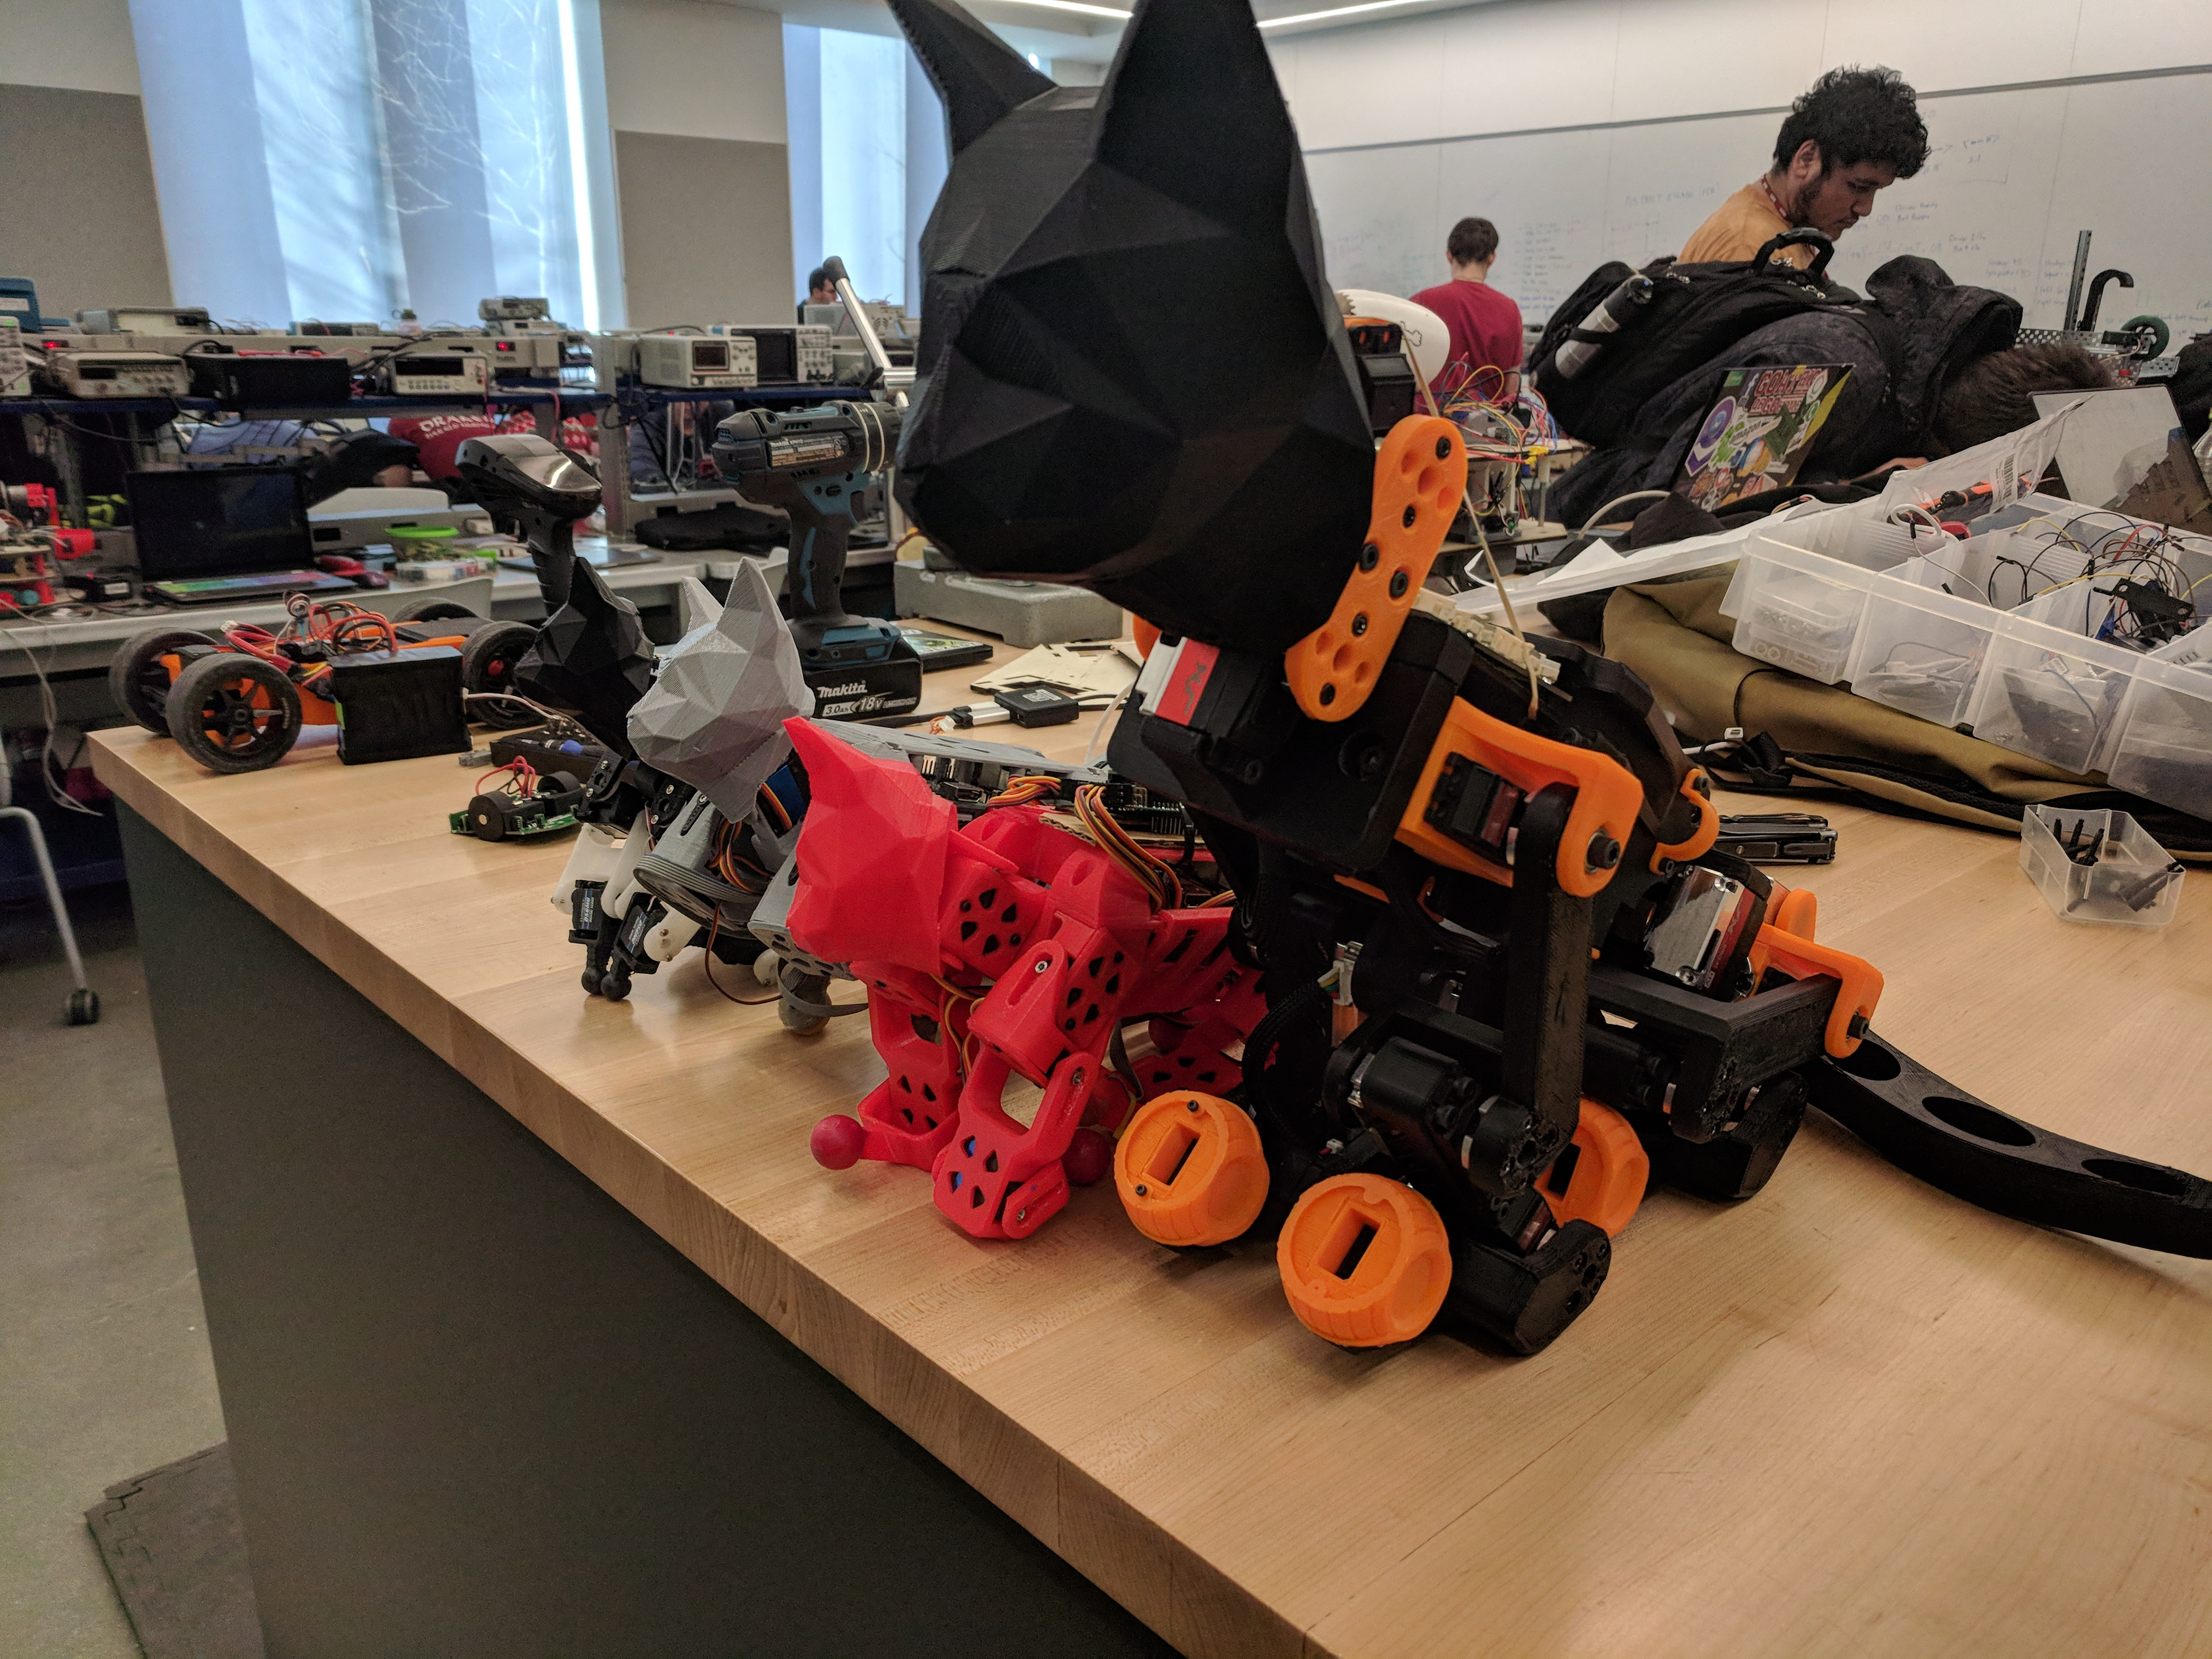
\includegraphics[width=0.5\textwidth]{figures/SmallKats.jpg}
                \caption{All four SmallKats posing for a picture}
                \label{fig:SmallKats}
        \end{figure}  
        
        \begin{figure}[H]
                \centering
                \includegraphics[width=0.5\textwidth]{figures/TestJig.jpg}
                \caption{Prototype 6 up on a custom test jig designed to support the cat during testing}
                \label{fig:TestJig}
        \end{figure} 


        \paragraph{Final Design}
        Using everything we had learned from our testing, design iterations and prototypes we were able to create a final design. This design was very similar to Prototype 6 with a few changes to the body and the leg design. Additionally it incorporated the continuum tail and had a few additional aesthetic pieces. Overall we were very pleased with the final mechanical design. It was sleek, functional, compact and looked good. 
         
         \begin{figure}[H]
                \centering
                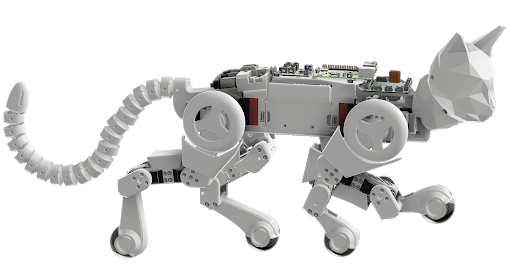
\includegraphics[width=0.5\textwidth]{figures/FinalDesign.png}
                \caption{Rendering of the Final Design}
                \label{fig:FinalDesign}
        \end{figure} 

         \begin{figure}[H]
                \centering
                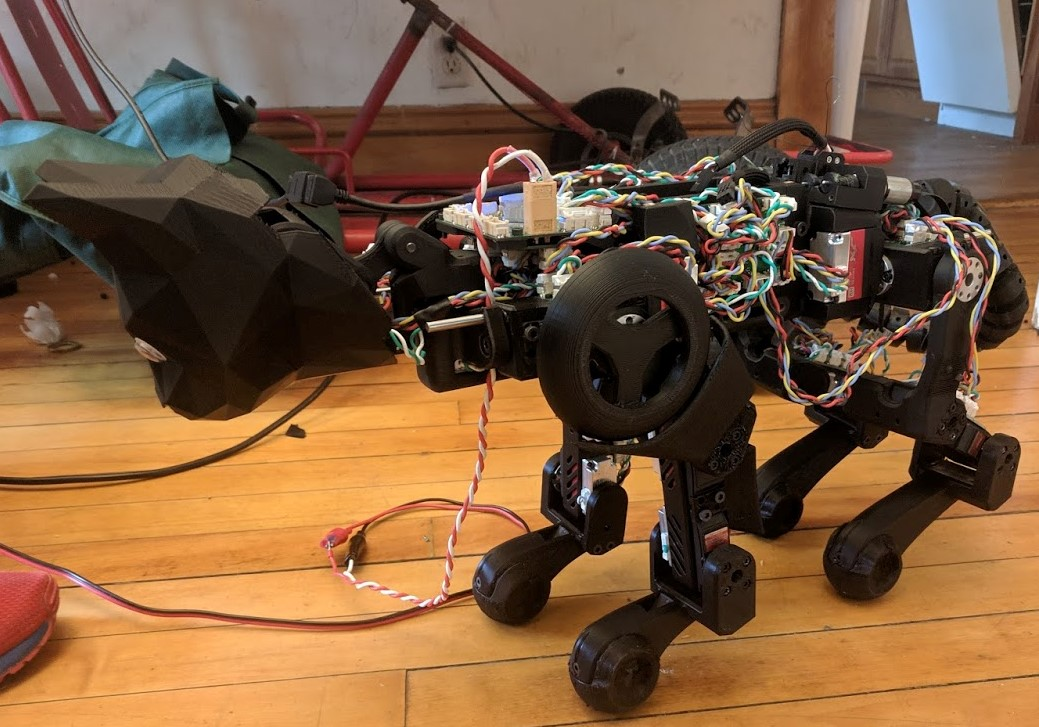
\includegraphics[width=0.5\textwidth]{figures/TestingFinalDesign.jpg}
                \caption{Fully assembled final design standing powered under own weight}
                \label{fig:TestingFinalDesign}
        \end{figure} 

\subsection{Electrical}
\subsubsection{Low-Level Control Software} 
    The low level control software of the robot can be broken down into four distinct subcategories. These include the master controller, foot sensors, motors and IMUs. 
        \subsubsection{Communication Structure}
        When the motherboard receives trajectory points from the computer over USB HID, the controller then parses the data received to each motor. This controller performs calculations in order to optimize leg trajectory and paths. The data is packaged into four byte packets shown below.  
        \begin{figure}[H]
        \centering
        \begin{tabular}{|c|c|c|c|c|}
        \hline
        Device ID& Command & Val 1 & Val 2 & Val 3\\
        \hline
        \end{tabular}
        \caption{Data packet structure}
        \label{fig:DataPacketStructure}
        \end{figure}
        The data is then sent to the motors, foot sensors and any other devices connected in the chain. Due to the nature of the system the data must be sent in order of the last device first as shown below. 
        \begin{figure}[H]
        \centering
        \begin{tabular}{|c|c|c|c|c|}
        \hline
            Foot Sensor & Motor 4 & Motor 3 & Motor 2 & Motor 1  \\
            \hline
        \end{tabular}
        \caption{Order of packets sent to a leg}
        \label{fig:PacketOrder}
        \end{figure}
        The path of data follows the structure below.\newpage
        \begin{longtable}{|r|p{0.9\textwidth}|}
        \hline
        Packet & Action of data\\
        \hline
        {Packet 1} &  {\begin{itemize}
                        \item Motor 1 Receives the Foot Sensor packet, replies previous position, velocity and torque to motor 2
                        \item Motor 2 Receives return data from Motor 1 and replies its data to Motor 3
                        \item Motor 3 Receives return data from Motor 2 and replies its data to Motor 4 
                        \item Motor 4 Receives return data from Motor 3 and replies its data to the foot sensor 
                        \item The foot Sensor Receives return data from Motor 4 and replies the readings from the pressure sensors to the master controller
                    \end{itemize}}\\
                    \hline
        {Packet 2} &  {\begin{itemize}
                        \item Motor 1 Receives the Motor 4 packet, replies the Foot Sensor packet to motor 2
                        \item Motor 2 Receives the Foot Sensor packet and replies Motor 1 data to Motor 3
                        \item Motor 3 Receives return data from Motor 1 and replies Motor 2 data to Motor 4 
                        \item Motor 4 Receives return data from Motor 2 and replies Motor 3 data to the foot sensor 
                        \item The foot Sensor Receives return data from Motor 3 and replies Motor 4 data to the master controller
                    \end{itemize}}\\
                    \hline
        {Packet 3} &  {\begin{itemize}
                        \item Motor 1 Receives the Motor 3 packet, replies the Motor 4 packet to motor 2
                        \item Motor 2 Receives the Motor 4 packet and replies the Foot Sensor packet to Motor 3
                        \item Motor 3 Receives the Foot Sensor packet and replies Motor 1 data to Motor 4 
                        \item Motor 4 Receives return data from Motor 1 and replies Motor 2 data to the foot sensor 
                        \item The foot Sensor Receives return data from Motor 2 and replies Motor 3 data to the master controller
                    \end{itemize}}\\
                    \hline
        {Packet 4} &  {\begin{itemize}
                        \item Motor 1 Receives the Motor 2 packet, replies the Motor 3 packet to motor 2
                        \item Motor 2 Receives the Motor 3 packet and replies the Motor 4 packet to Motor 3
                        \item Motor 3 Receives the Motor 4 packet and replies Motor 1 data to Motor 4 
                        \item Motor 4 Receives the Foot Sensor packet and replies Motor 1 data to the foot sensor 
                        \item The foot Sensor Receives return data from Motor 1 and replies Motor 2 data to the master controller
                    \end{itemize}}\\
                    \hline
        {Packet 5} &  {\begin{itemize}
                        \item Motor 1 Receives the Motor 1 packet, replies the Motor 2 packet to motor 2
                        \item Motor 2 Receives the Motor 2 packet and replies the Motor 3 packet to Motor 3
                        \item Motor 3 Receives the Motor 3 packet and replies Motor 4 packet to Motor 4 
                        \item Motor 4 Receives the Foot Sensor packet and replies Motor 1 data to the foot sensor 
                        \item The foot Sensor receives Foot Sensor packet and replies Motor 1 data to the master controller
                    \end{itemize}}\\
        \hline
        \end{longtable}

        \noindent Once the cycle is completed the motors update the PID controllers, the foot sensors collect the pressure data and the cycle is looped. The return packet order is shown below.
        \begin{figure}[H]
        \centering
        \begin{tabular}{|c|c|c|c|c|}
        \hline
            Motor 1 & Motor 2 & Motor 3 & Motor 4 & Foot Sensor \\
            \hline
        \end{tabular} 
        \caption{Order of Data returned from a leg}
        \label{fig:DataReturnOrder}
        \end{figure}

        \paragraph{Motor Controllers}
            When the motor receives a packet it checks if the first byte if the packet and compares it to the device ID of the motor. If the device Id does not match the first byte of the packet it is stages for transmission on the next packet received. If the packet is used to update that motor, the second byte of the packet is checked and compared to different known options. 
            \begin{table}[H]
                \centering
                \begin{tabular}{|c|c|}
                \hline
                    Value & Command \\
                    \hline
                    0x22 & Update device ID based on byte 3 of the packet\\
                    0x47 & Updates Position PID constants based on bytes 3,4,5 of the packet \\
                    0x48 & Updates Velocity PID constants based on bytes 3,4,5 of the packet \\
                    0x49 & Updates Torque PID constants based on bytes 3,4,5 of the packet \\
                    0x91 & Updated position set point in Position PID loop\\
                    0x92 & Updated position set point in Velocity PID loop\\
                    0x93 & Updated position set point in Torque PID loop\\
                    \hline
                    \end{tabular}
                \caption{Command values for motors}
                \label{tab:ServoCommandValues}
            \end{table}
            In between receiving packets the motors run multiple PID loops simultaneously to control position, torque and velocity at greater than  a 10kHz refresh rate.
        \paragraph{IMU}
            The IMU micro controller continuously samples the BNO055, recording the current gyroscope, acceleration and magnetometer data. On request from the master controller the IMU checks byte 1 and compares it to the device ID, if it matches it compares byte 2 to the list of known commands and replies accordingly which can be see below.
            \begin{table}[H]
                \centering
                \begin{tabular}{|c|c|}
                \hline
                    Value & Command \\
                    \hline
                    0x22 & Update device ID based on byte 3 of the packet\\
                    0x37 & get gyroscope data\\
                    0x38 & get accelerometer data\\
                    0x39 & get magnetometer data\\
                    \hline
                    \end{tabular}
                \caption{Command values for IMU}
                \label{tab:IMUCommandValues}
            \end{table}

        \paragraph{Foot Sensor}
            Similarly to the IMU, the foot sensor micro controller continuously samples the 7 pressure sensors. On request from the master controller the foot sensor checks byte 1 and compares it to the device ID, if it matches it compares byte 2 to the list of known commands and replies accordingly which can be see below.
            \begin{table}[H]
                \centering
                \begin{tabular}{|c|c|}
                \hline
                    Value & Command \\
                    \hline
                    0x22 & Update device ID based on byte 3 of the packet\\
                    0x32 & return most recent foot pressure sensor readings\\
                    \hline
                    \end{tabular}
                \caption{Command values for foot sensor}
                \label{tab:FootSensorCommandValues}
            \end{table}

\subsubsection{Motors}
The custom servo motors posed a very interesting challenge when it came to size and component density. On a board that had to fit in an 18mmx36mm space a micro controller, magnetic encoder, voltage regulator, 2 connectors, a motor driver and a motor along with all supporting circuitry. This along with some simple oversights meant the board went through 2 major revisions and 1 minor revision. 

\begin{figure}[H]
       \centering
       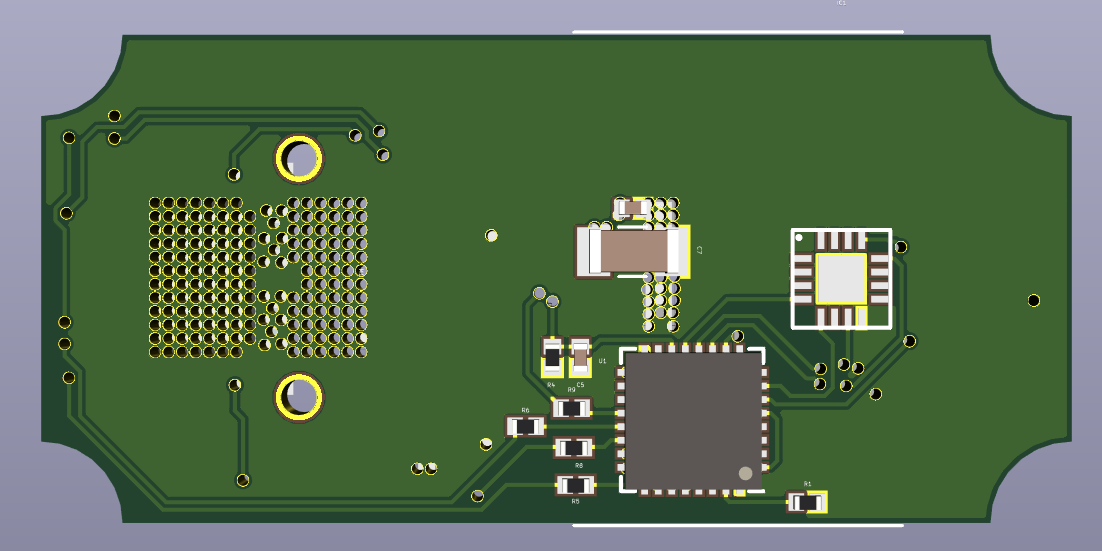
\includegraphics[width=0.6\textwidth]{figures/MotorControllerBottom.png}
       \caption{Motor controller PCB bottom}
       \label{fig:MotortControllerPCBBottom}
   \end{figure}
   \begin{figure}[H]
       \centering
       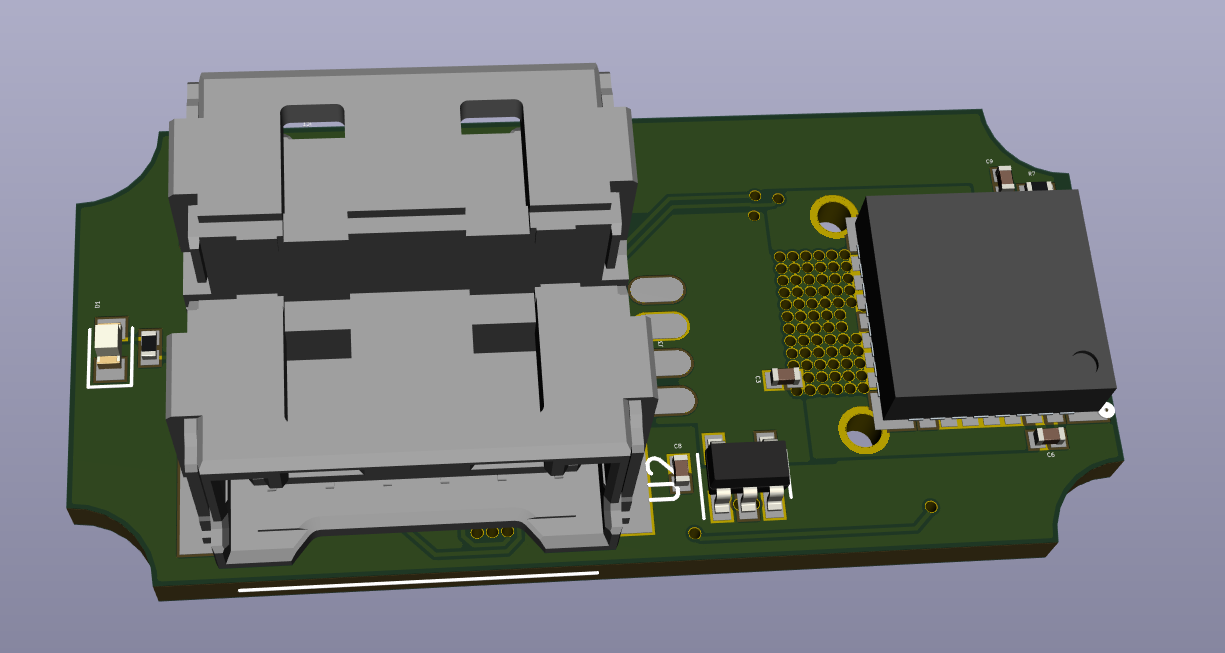
\includegraphics[width=0.6\textwidth]{figures/MotorControllerTop.png}
       \caption{Motor controller PCB top}
       \label{fig:MotorControllerPCBTop}
   \end{figure}
The boards were designed to be assembled directly into the motor connected directly by the motor pins, aligning the encoder above the magnet connected directly to the output shaft of the motor. The programming header was designed as a series of pads that can be used in combination with a Pogo pin programming jig, meaning that the firmware can be updated quickly and easily. 
\subsubsection{Motherboard}
The mother board was developed to be a stand alone micro controller using the STM32H743vit6 micro controller running at 400 MHz. Broken out from this micro controller were all 6 SPI channels, 12 GPIO pins, UART, USB HS and a programming header. In order to limit the number of traces interfering with the High power  coming from the battery, 3.3v and the Ground Plane a 4 layer board was chosen despite the increased cost of production. This meant that all the signal traces could be run internally allowing for a continuous trace running around the periphery of the board connecting all of the connectors to the 8.4v supply coming in from the battery.
\begin{figure}[H]
       \centering
       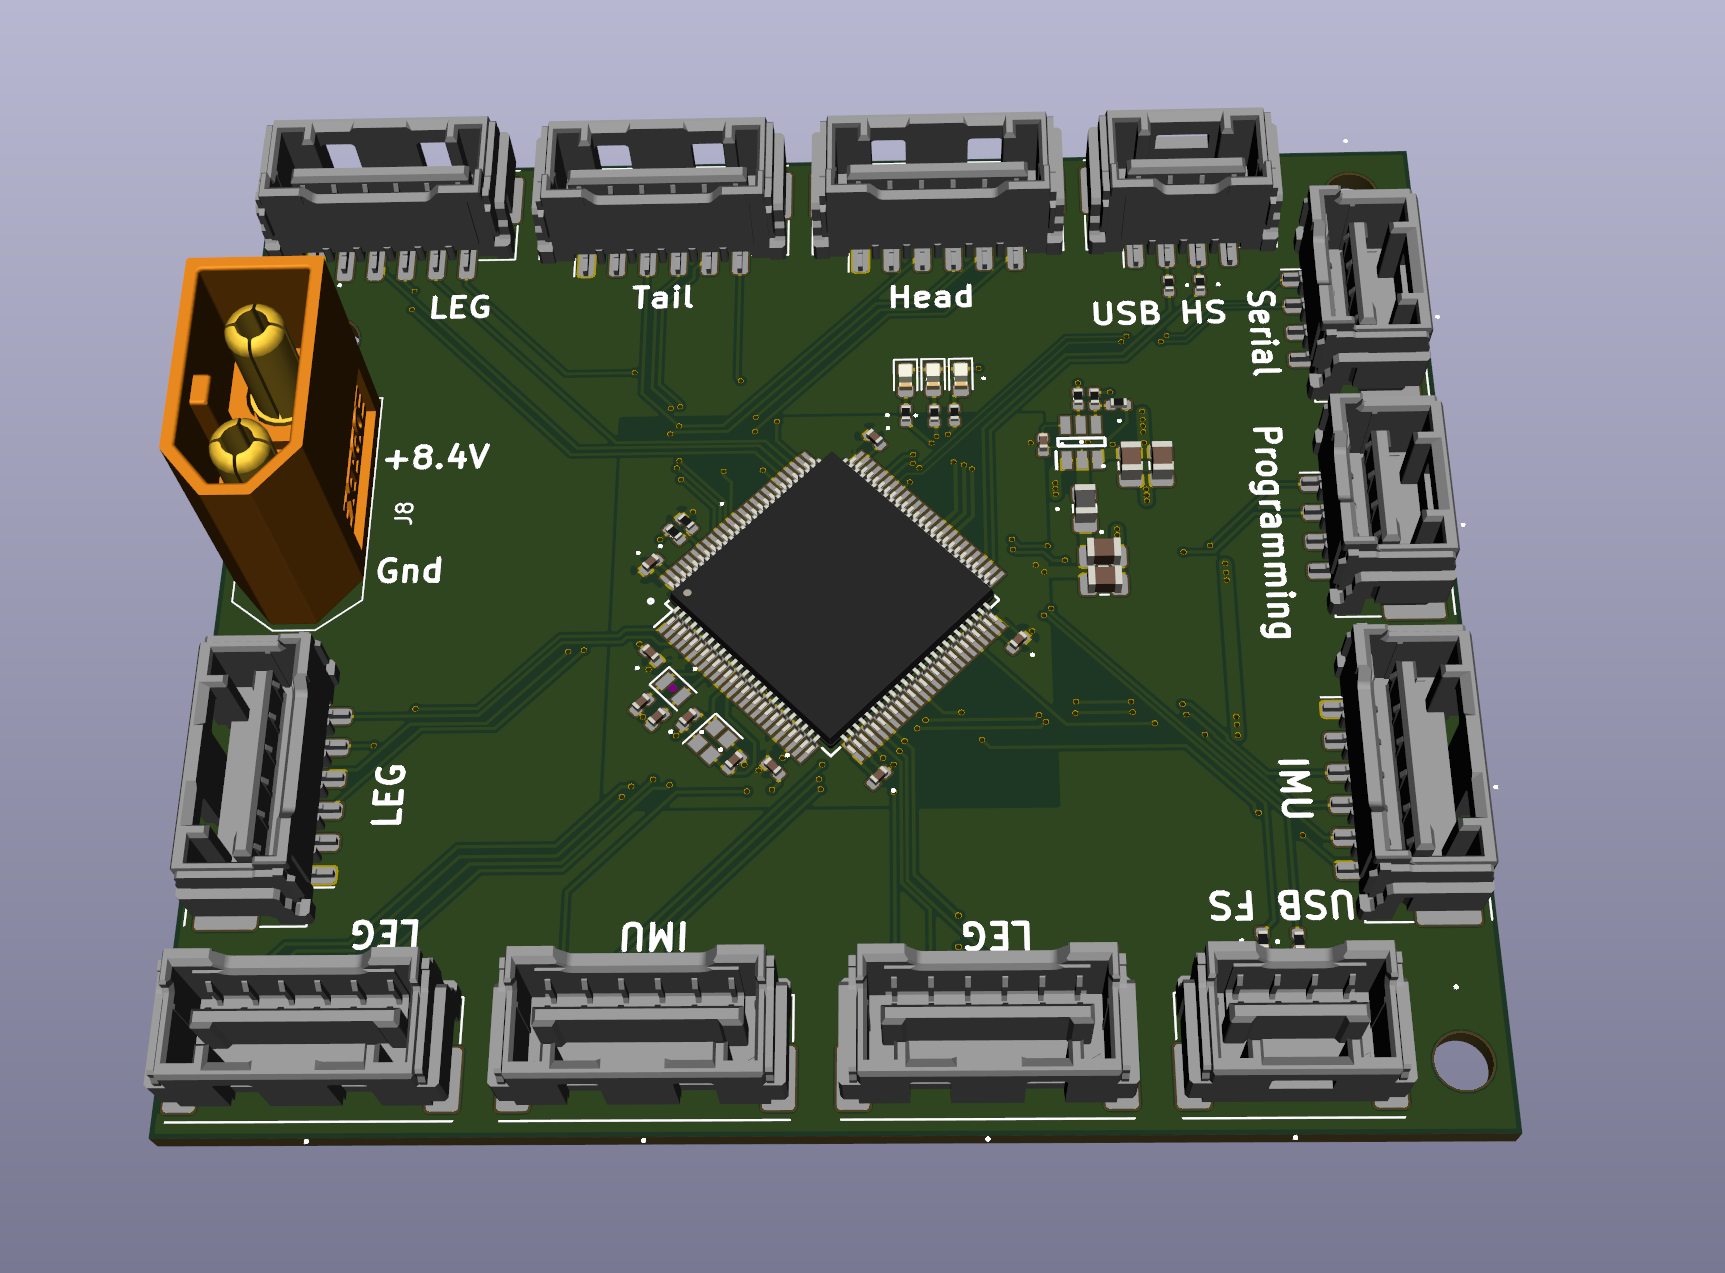
\includegraphics[width=0.6\textwidth]{figures/Motherboard_Rev2.png}
       \caption{Motherboard}
       \label{fig:MotherboardPCB}
   \end{figure}
To ensure reliability at higher clock speeds both a 32.768 kHz crystal oscillator and a 32MHz crystal oscillator were used. While developing the firmware for the motherboard the the clock speed was reduced from 400MHZ to 384 MHz in order to optimize the speed at which the SPI could be run as a clock divisible by 24MHz was requires to take full advantage of the SPI communication with the micro controllers on the motors. In order to have a reliable and stable 3.3v rail for the micro controller, 2 switch mode buck converter power supplies were used in order to stop regulate the 5v supply from USB and the 8.4v supply from the battery pack. This allows the board to be developed on and tested using only power from the USB connection and does not require the battery be connected. 
  
   The motherboard was designed and went through one minor and one major, the minor revision was done to remedy an error in the switch mode power supply circuit as well as to change from USB FS to USB HS allowing for a much faster data  through put at up to 480Mb/s.
 	The Major revision was done in order to switch micro controllers to a micro controller package much better suited for the application. Instead of using the 176 pin package of micro controller, the 100 pin variant was capable of performing the same tasks required. In addition to the change in micro controller, Both available USB ports were broken out and much more safe guarding against inductive spikes affecting the master micro controller were implemented due to the death of 2 of the previous revision. Though many of these changes were very beneficial, the changing of microcontrollers came with a single draw back, the loss of 1 SPI channel, meaning some motors were forces to share SPI channels with other devices on the robot. This prevented us offloading the processing of SPI data to the hardware DMA as it had the possibility of cross talk between multiple devices. The breaking out of both USB ports did allow us to take advantage of the processing power and speed of the micro controller. By combining both ports we were effectively able to double our throughput, sending data and requests for different devices through different ports. Using the USB HS ports for motor data and the USB FS port primarily for IMU data requests allowed us to remove the bottle neck of having to wait for the data transmission to be completed and allowed us to increase the sample rate of the IMU.
\subsubsection{IMU}
\begin{figure}[H]
       \centering
       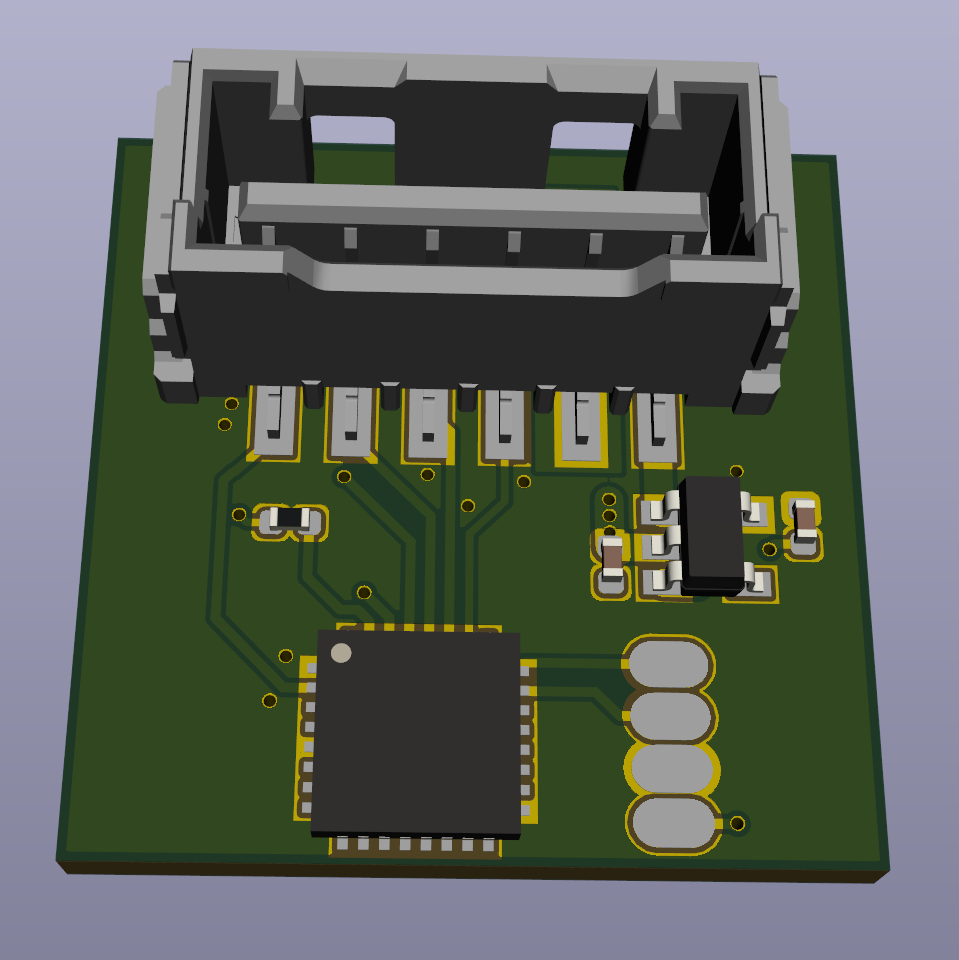
\includegraphics[width=0.5\textwidth]{figures/IMU.png}
       \caption{IMU Breakout}
       \label{fig:IMUPCB}
   \end{figure}
   The IMU breakout allows a BNO055 IMU to be used as any other device in the system, Using the same communication protocol and similar command IDs as the motors, charger, tail controller and other boards in the system. The board continuously samples the BNO055 IMU for Accelerometer, Gyroscope and Euler angles for heading, roll and pitch and on a request for data responds with all 9 of these data sets from the most recent update.This reduces the data request time for the master controller drastically as this IMU is notorious for clock smearing on i2c and having long delays between samples.
   
\subsubsection{Foot Sensors}
\begin{figure}[H]
       \centering
       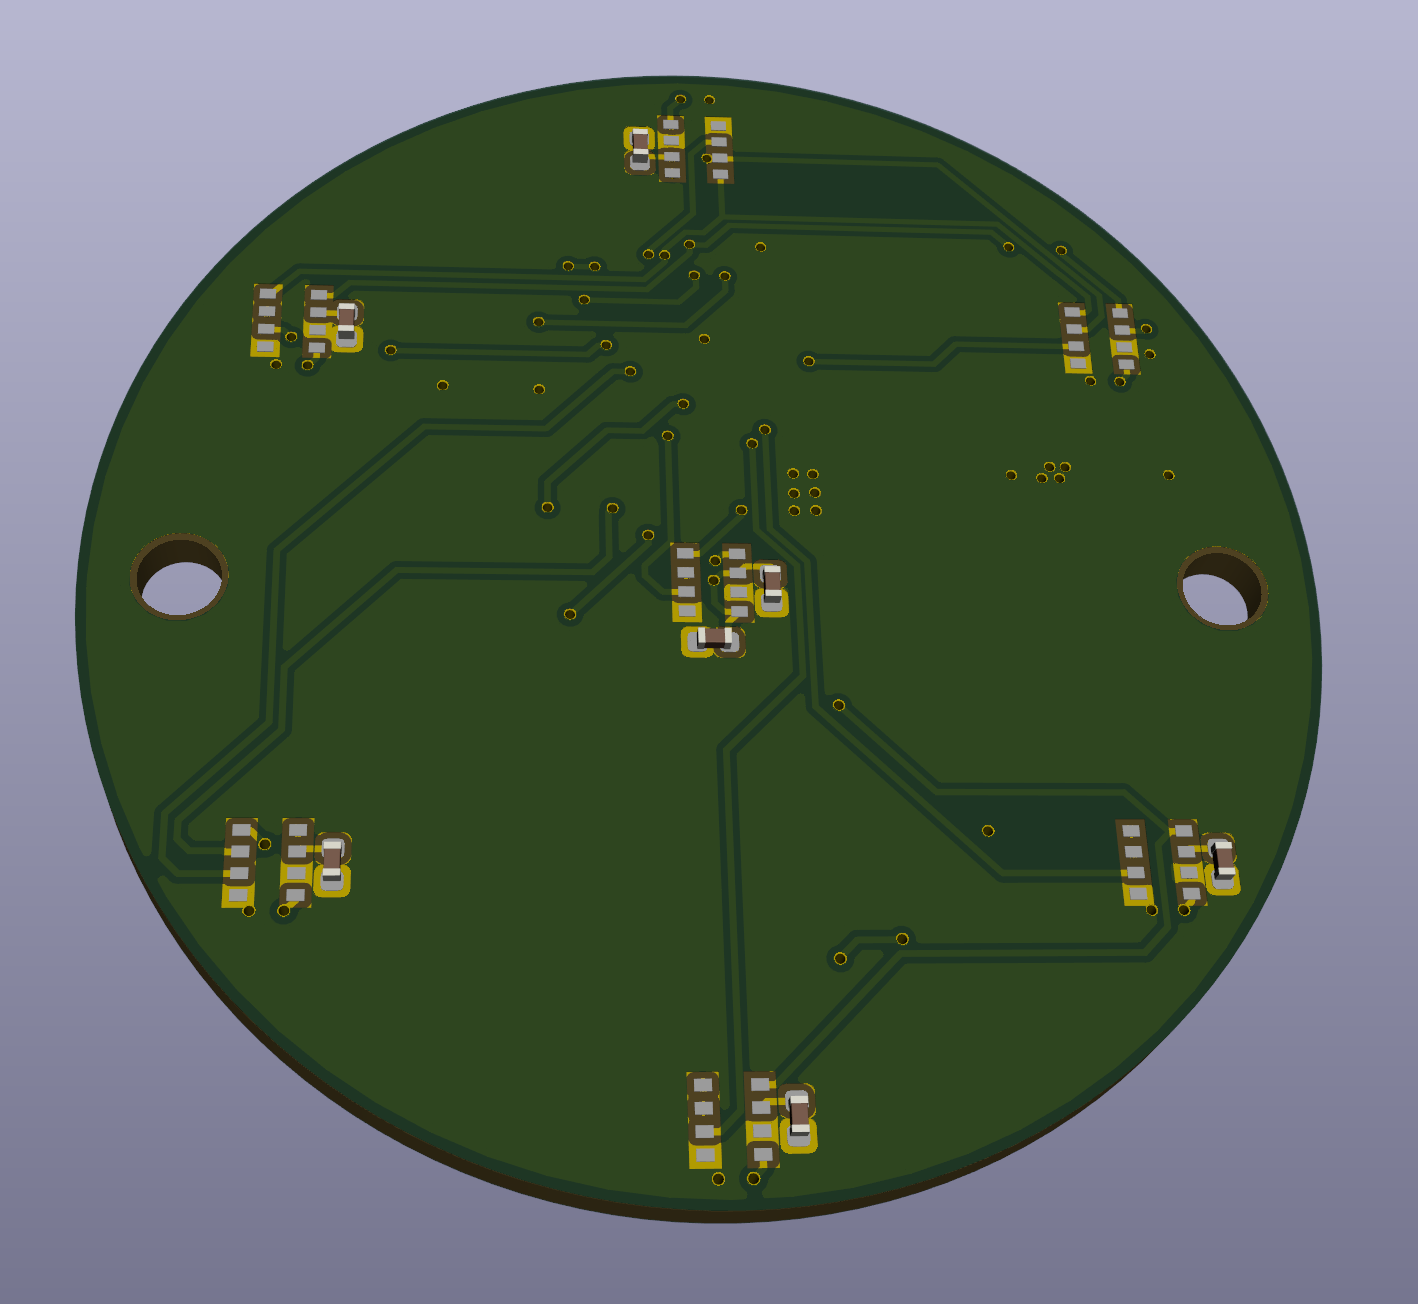
\includegraphics[width=0.5\textwidth]{figures/FootSensor.png}
       \caption{Foot Sensor}
       \label{fig:FootSensorPCB}
   \end{figure}
\paragraph{Board Design}
\subparagraph{Vector Triangulation}
Many means of calculating the location of the pressure vector were considered however many of them were unreliable and/or difficult to implement on a micro controller using C/C++. This led us to developing a triangulation algorithm similar to that used by police to triangulate a cell phone based on near by cell towers. The pressure of the sensors in a quadrant(one sector of the total sensor) is read and the equations of 3 circles with pressure dependent radius are calculated, the higher the pressure read the smaller the radius of the circle. The intersection points of the circles are then calculated and the equations of 3 lines are found and the intersection point of all three of those is found. This gives the center point of the pressure centroids. 
\begin{figure}[H]
    \centering
    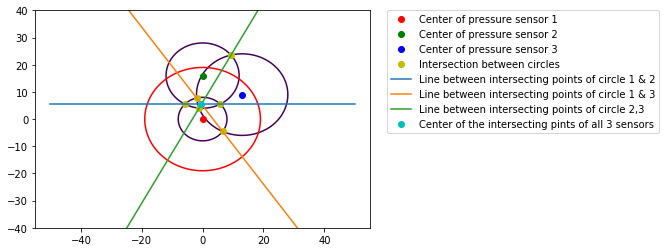
\includegraphics[width=0.8\textwidth]{figures/Triangulation.png}
    \caption{Pressure Vector Triangulation}
    \label{fig:PressureVectorTriangulation}
\end{figure}
This location in XY is then extrapolated to the position on the foot by calculating its Z location based on the equation of the sheer created by the casting. The magnitude of the force can also be calculated by the absolute additional pressure introduced to the system by finding out the amount of pressure being applied to all the sensors and removing that from the calculations. essentially finding the minimum pressure that must be applied at each sensor to intersect at that point.
\begin{figure}[H]
    \centering
    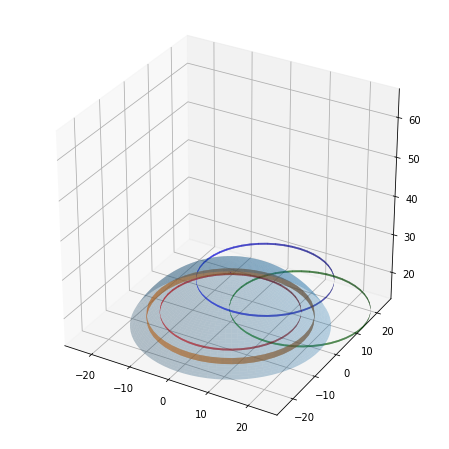
\includegraphics[width=0.6\textwidth]{figures/Footsensordome.png}
    \caption{3D Pressure Vector Triangulation}
    \label{fig:3DPressureVectorTriangulation}
\end{figure}

\subsubsection{Charger}
\begin{figure}[H]
       \centering
       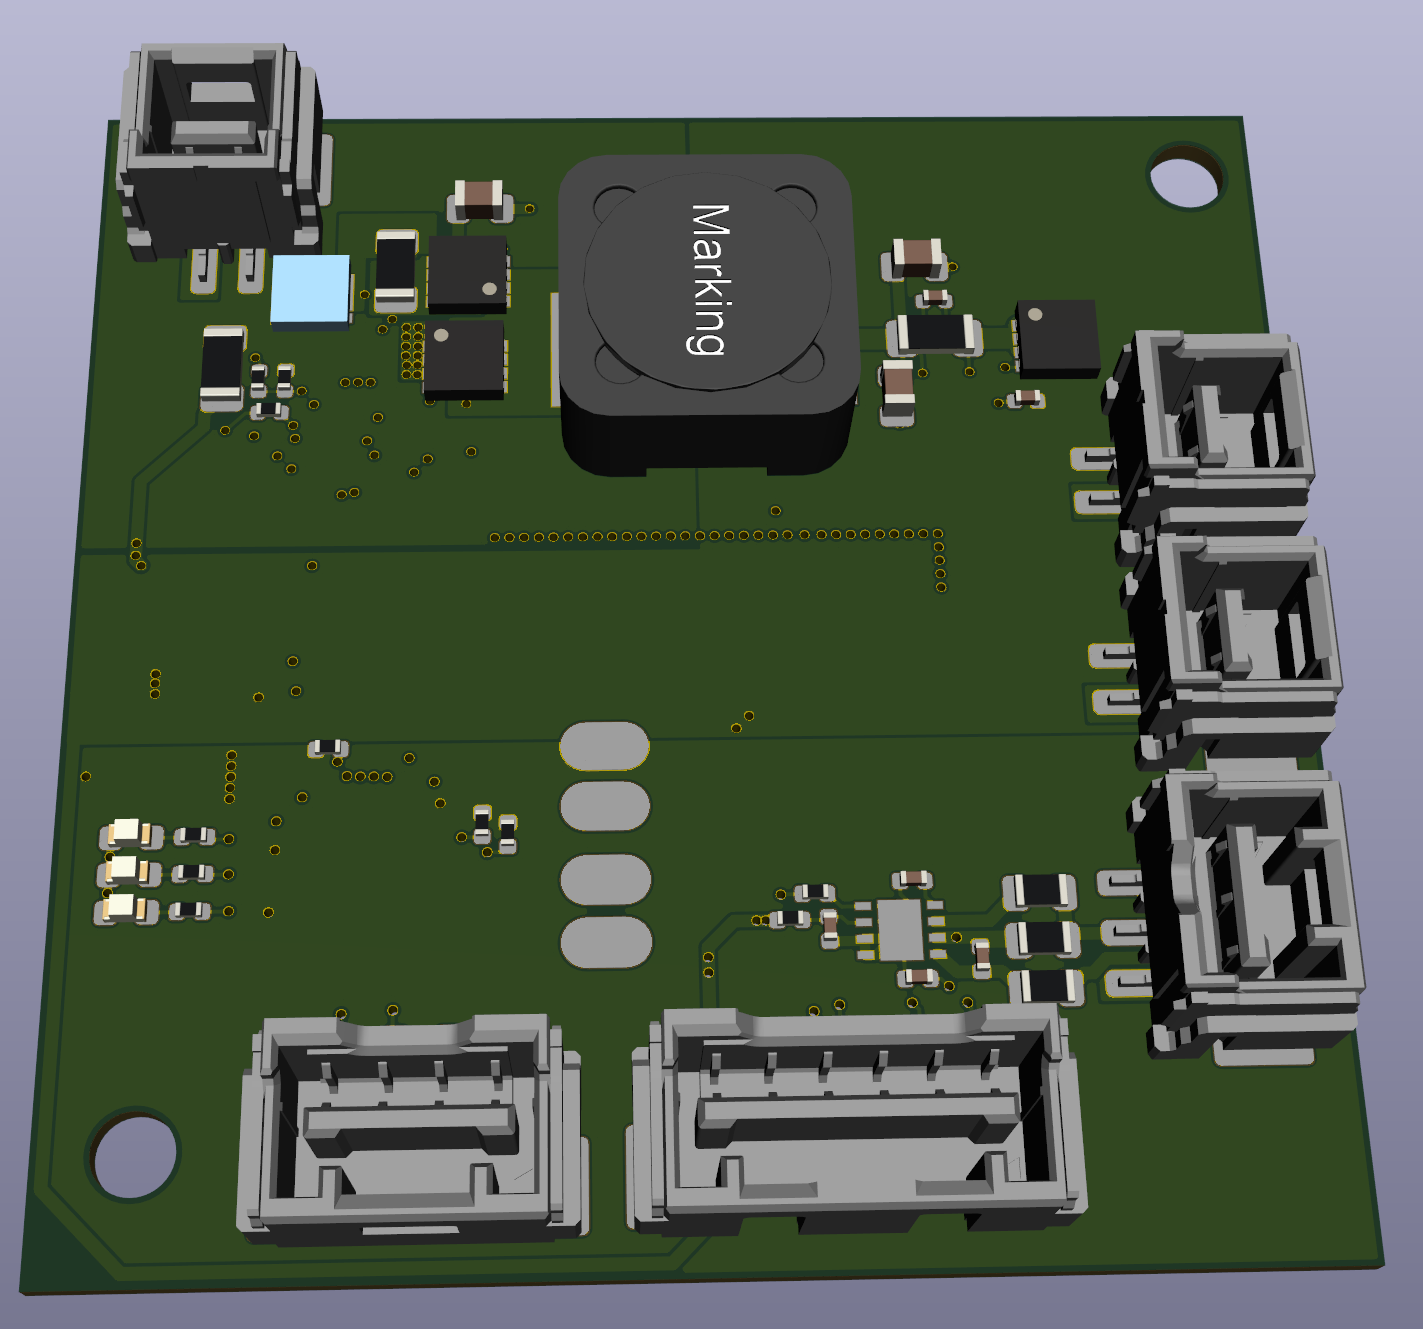
\includegraphics[width=0.5\textwidth]{figures/Charger.png}
       \caption{Battery Charger}
       \label{fig:ChargerPCB}
   \end{figure}
The development of this charging board allows us to fine tune the charge voltage and charge current of the battery back. This board also allows us to monitor the battery voltage and prevent over discharging as well as balancing the cells at all times. The voltage is constantly being monitored and reported to the motherboard. This allows the system to stop allowing motor updates at a given voltage cutoff point. This safety feature will help to prevent over draw from the batteries diminishing the available capacity of the pack. The charging current is able to be fine tuned up to 8A using BQ24715 charging IC from TI. The charging voltage and current can be updated on the fly through the SMbus interface. The BQ29200 balance charging IC allows for the batteries to be balanced continually ensuring the cells never go out of sync, ensuring longevity of the pack.

\subsubsection{Tail Control Board}
\begin{figure}[H]
       \centering
       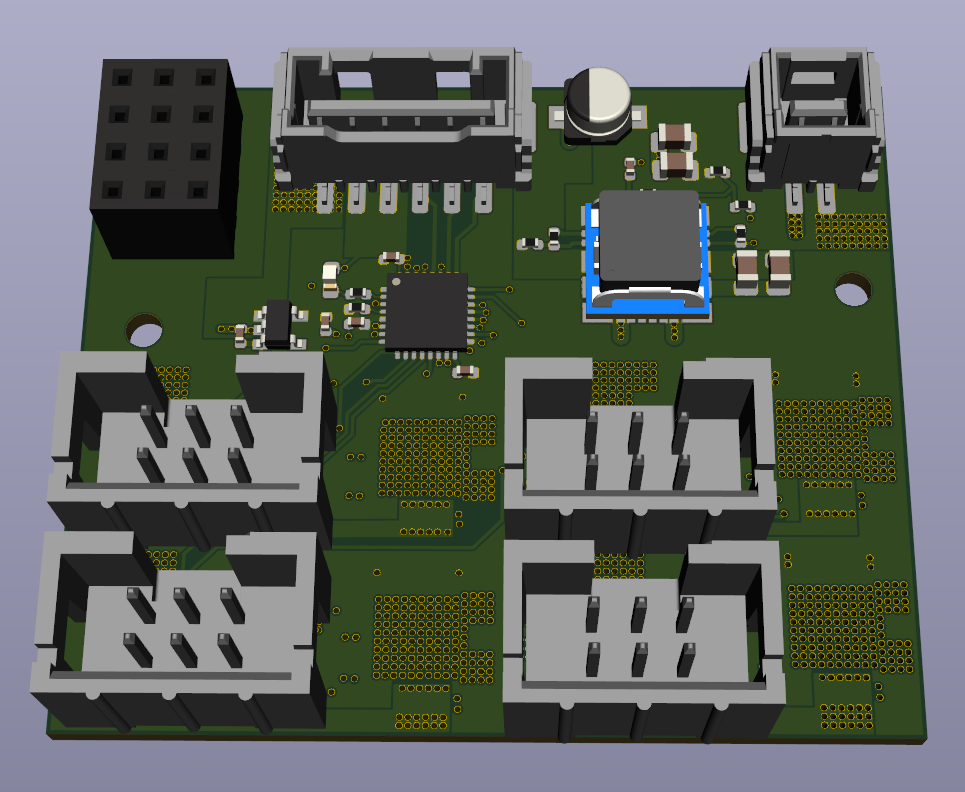
\includegraphics[width=0.5\textwidth]{figures/TailControllerBoard.png}
       \caption{Tail Motor Controller}
       \label{fig:TailControlBoardPCB}
   \end{figure}
   The intention of this board is to control the 4 Maxon A-Max motors being used to drive the continuum tail of the robot. In order to do this the board must facilitate the homing of the tail, in this case using limit switches, communicate with the motherboard to receive the set point of each motor and run all four PID controllers and keep track of the quadrature encoders for each motor, each having 4096 counts per revolution. This board is also being used to power the on board raspberry pi using an integrated inductor switch mode power supply from TI which is capable of providing up to 60W of power for the case that another SBC was chosen. 
   
\subsubsection{SPI to RS485 Converter Board}
\begin{figure}[H]
       \centering
       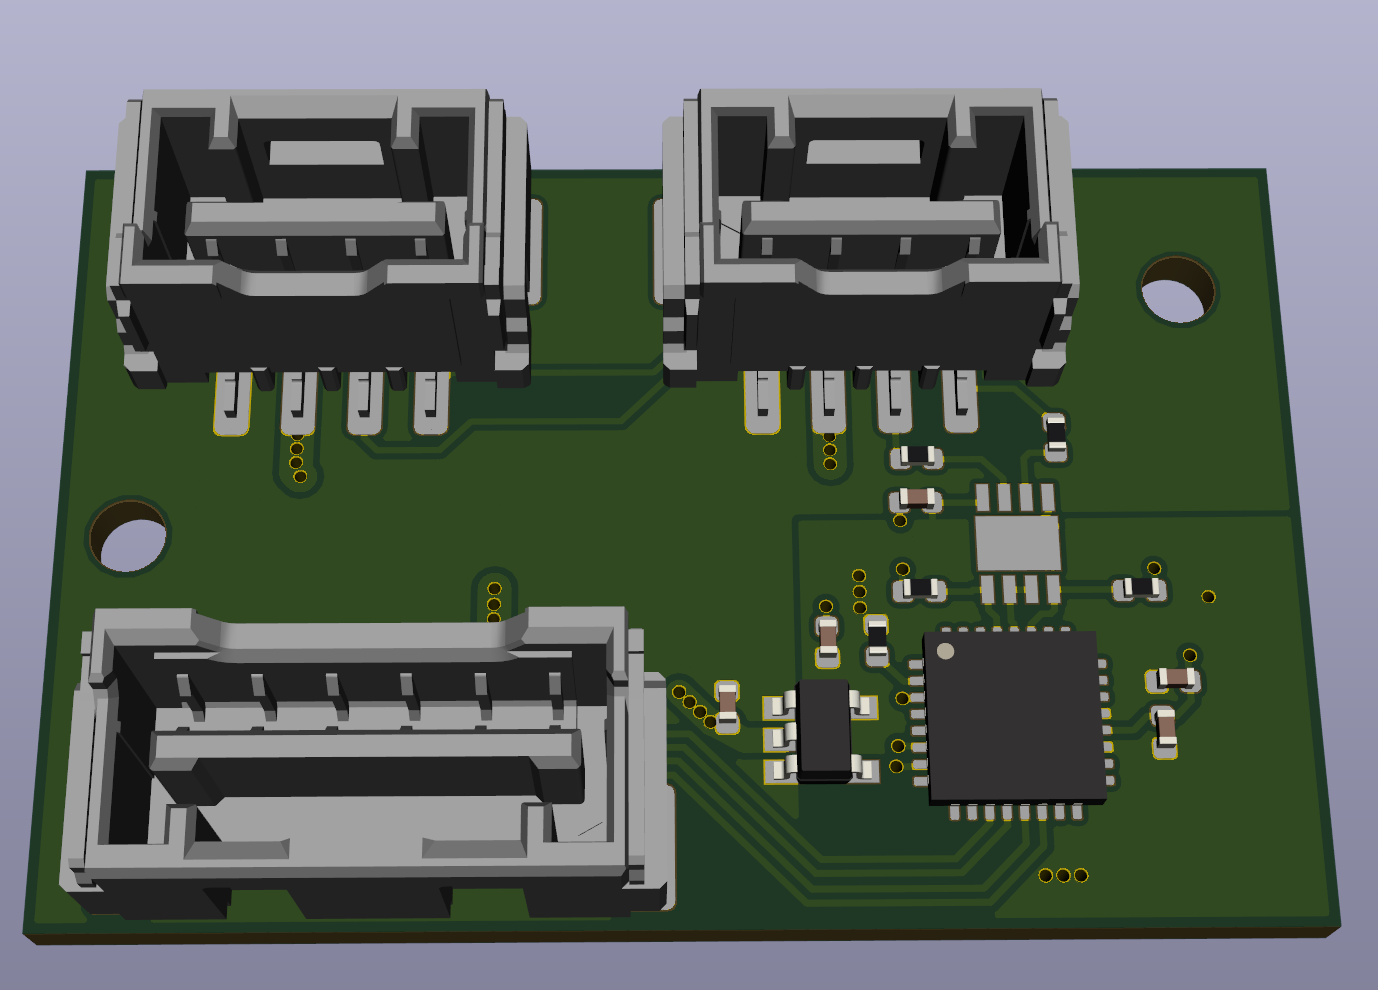
\includegraphics[width=0.5\textwidth]{figures/ConverterBoard.png}
       \caption{SPI to RS485 Converter}
       \label{fig:SPItoRS485ConverterPCB}
   \end{figure}
   After investing over 100 hours of debugging and testing into the daisy chained SPI protocol of the motors, it was found that The SPI lines were not always pulled completely high or completely low due to the number of devices sharing the same line, this combined with the noise that would be developed in the system and the propagation time between the data being passed between devices made the system very unreliable with 4 motors connected in a chain. A single motor would work 100\% of the time, 2 motors would work approximately 80\% of the time and decaying exponentially there after resulting in the fourth motor being extremely unstable and completely unreliable. This led to the decision to change from SPI to RS485. Due to time and cost constraints it was decided to leave the motors in the state they currently existed in and add external communication boards, 1 per motor. These boards would take the SPI signal from the motherboard, convert it to an RS485 differential signal that would be sent to all the daughter boards that if the message was meant for that board, would then transfer the data to the motors and the motor response back upstream to the master. This conversion proved to be much more stable dropping nearly 0 packets. This however came with a major drawback, the maximum UART speed of the chosen microcontrollers (LPC824) was only 1Mbit/sec, this combined with the removal of the synchronous protocol meant the re was an effective data transmission speed of only 500kbit/sec. Luckily through testing this proved to be a non issue due to the PID controllers being run locally and the update speed of the USB communications being limited by the computer to only 1kHz 

\subsubsection{Custom Battery Pack}
\begin{figure}[H]
       \centering
       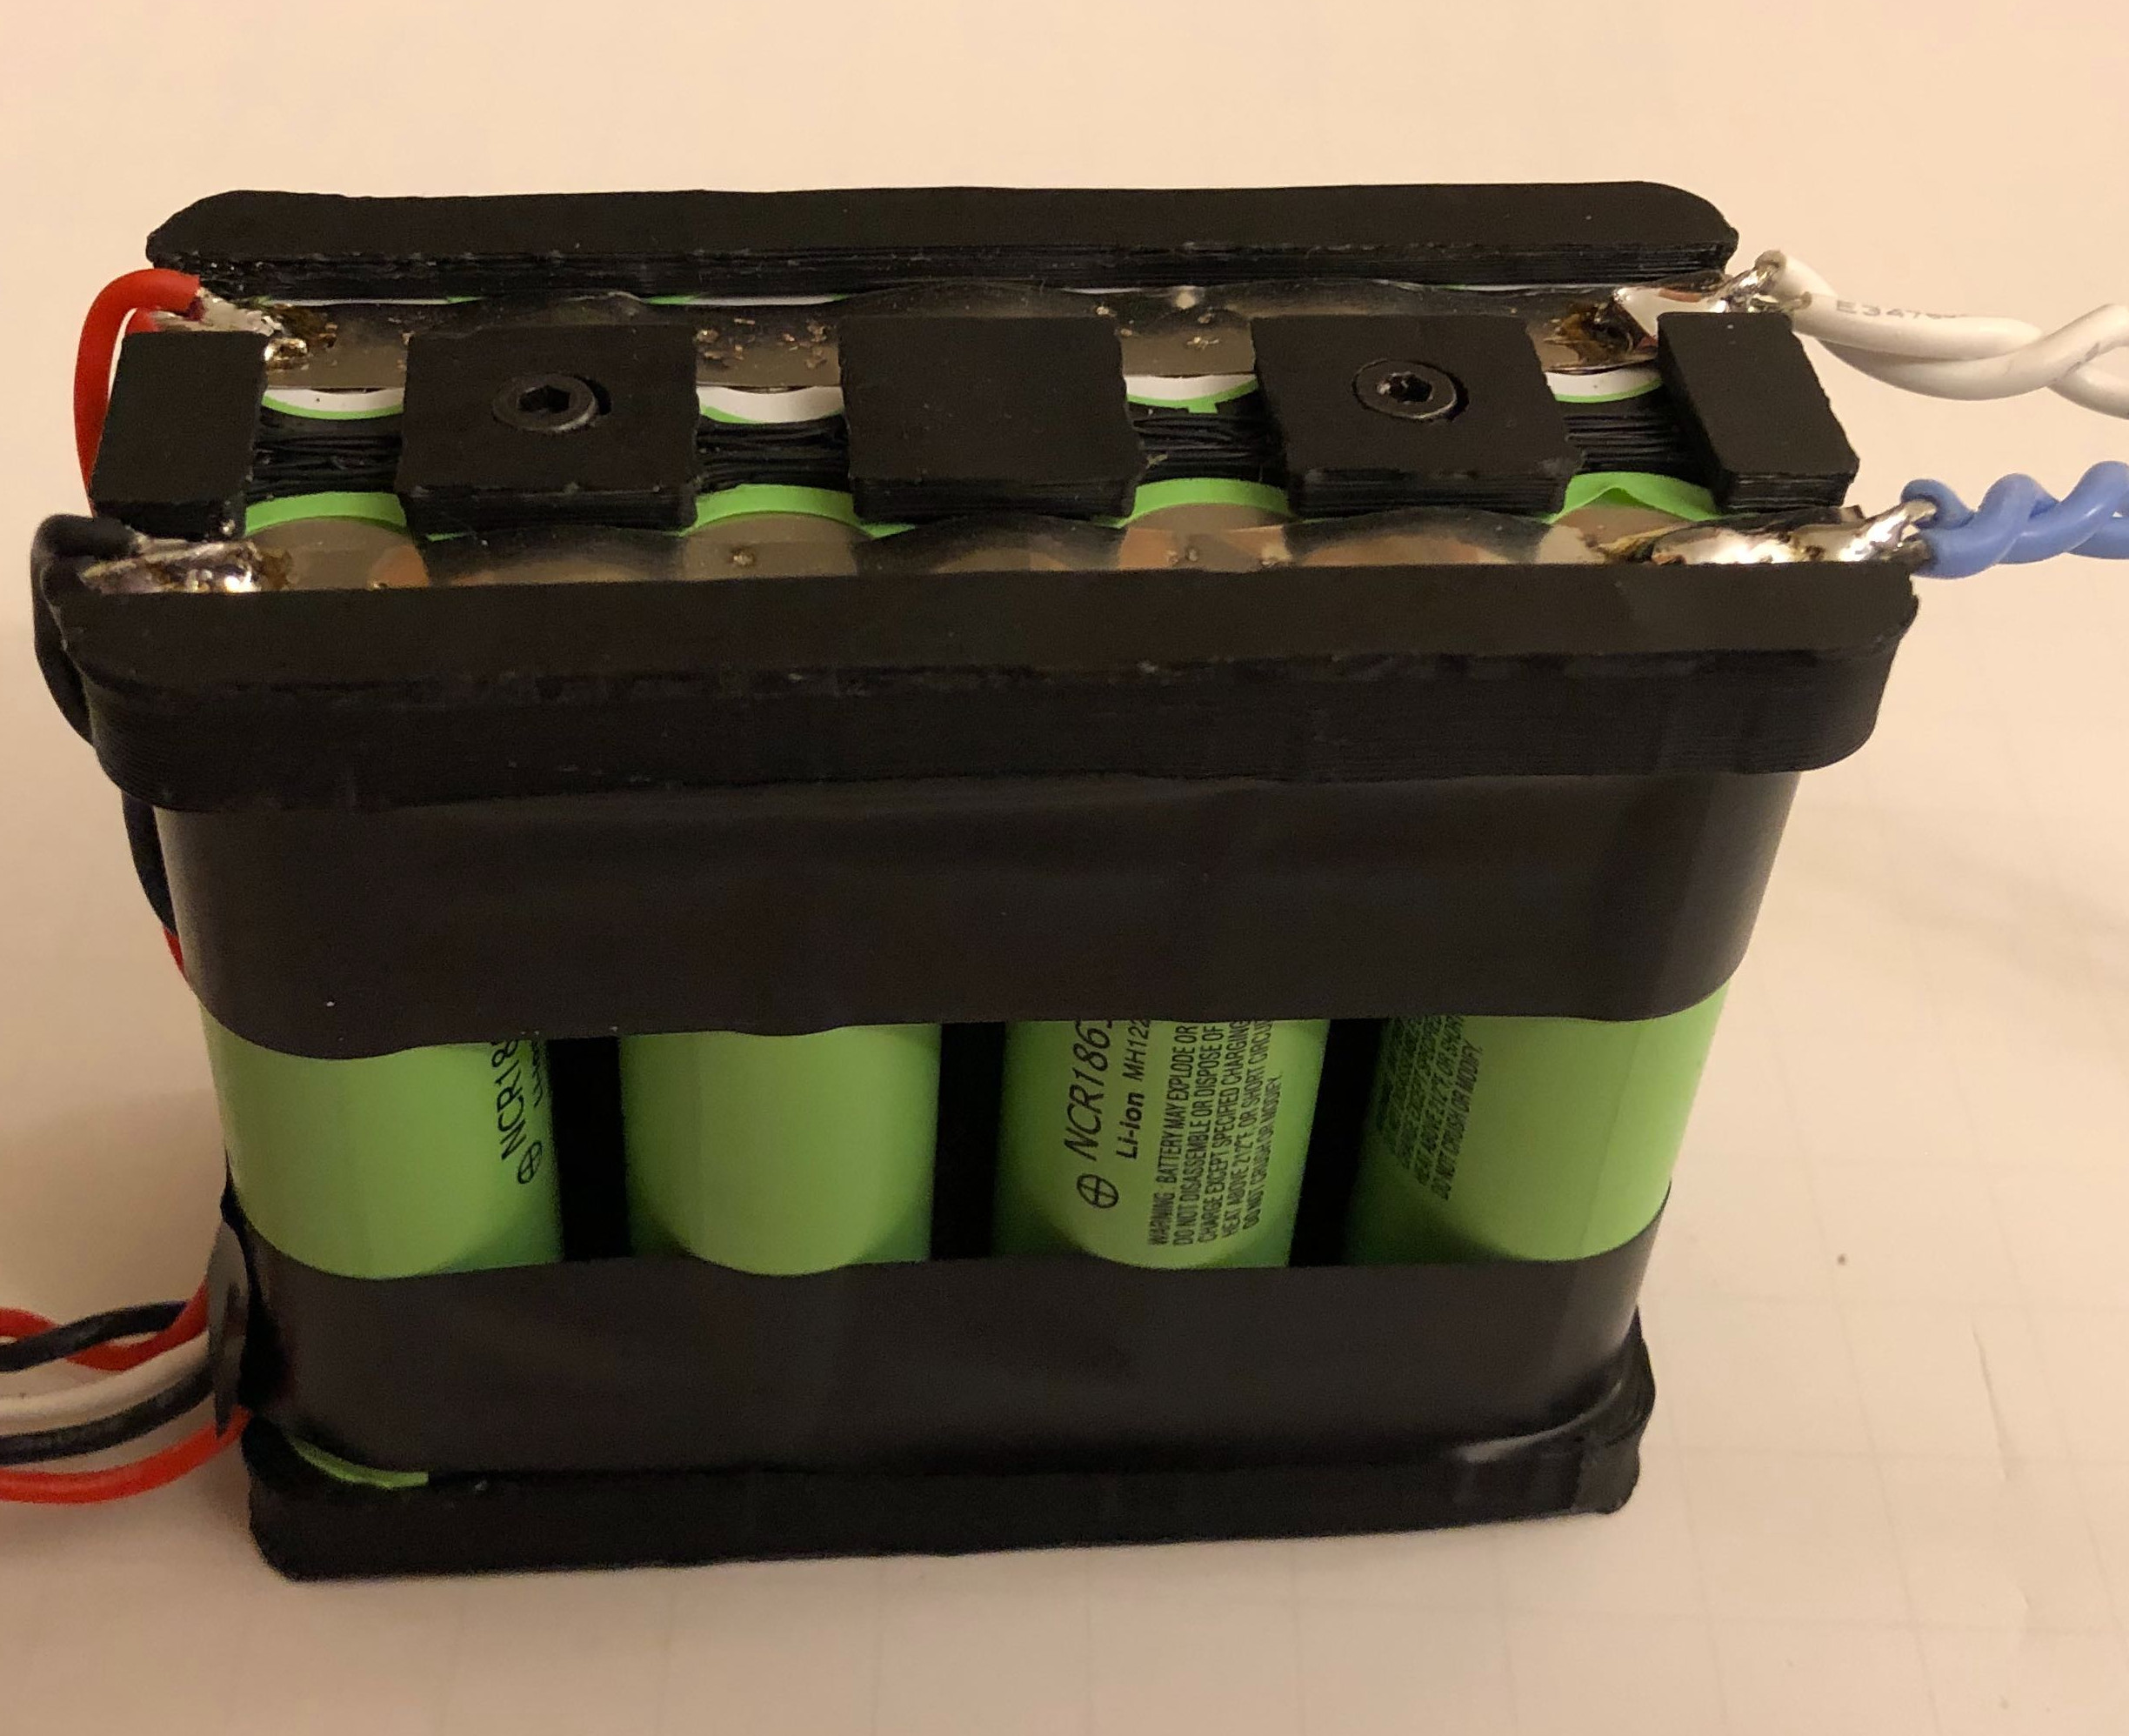
\includegraphics[width=0.4\textwidth]{figures/CustomBatteryPack.jpg}
       \caption{Custom Spot welded battery pack}
       \label{fig:CustomBatteryPack}
   \end{figure}
   After a lot of research the route of creating a custom battery pack made of Panasonic NCR18650B cells was chosen instead of purchasing a commercially available lithium polymer / lithium ion battery. This decision was made for a number of reasons;primarily due to the size and shape constraints of the robot. In order to get a battery pack that would fit in the space we would have to compromise on capacity. Another reason is in doing research Panasonic NCR18650B cells had one of the highest energy to weight ratios available on the market at 3400mAh at only 44g/cell. This allowed us to create a battery pack with a cumulative 13600mAh of power at a nominal 7.4V. This will allow to robot to operate in a walking state for approximately 1.5 hours.

\subsection{Software}
    As stated in Section \ref{subsec: Software}, the software platform chosen was Bowler Kernel, due to its familiarity and visualization capability. During development, we implemented and used a visualization tool to simplify graphics computation on the development machines and to visualize joint limits and DH parameters on the robot. When it came to running a headless system, we also switched from an Odroid XU4 to a Raspberry Pi 3 B+, due to limitations by Bowler Kernel. 
    
    \subsubsection{Visualization Simplification}
        When developing software, our team quickly figured out that rendering our complex CAD model for visualization would unnecessarily put computational strain on our computers. Therefore, we implemented a visualization tool that would allow us to look at the constraints of the robot. This included DH parameters, joint limits, and
        \begin{figure}
            \centering
       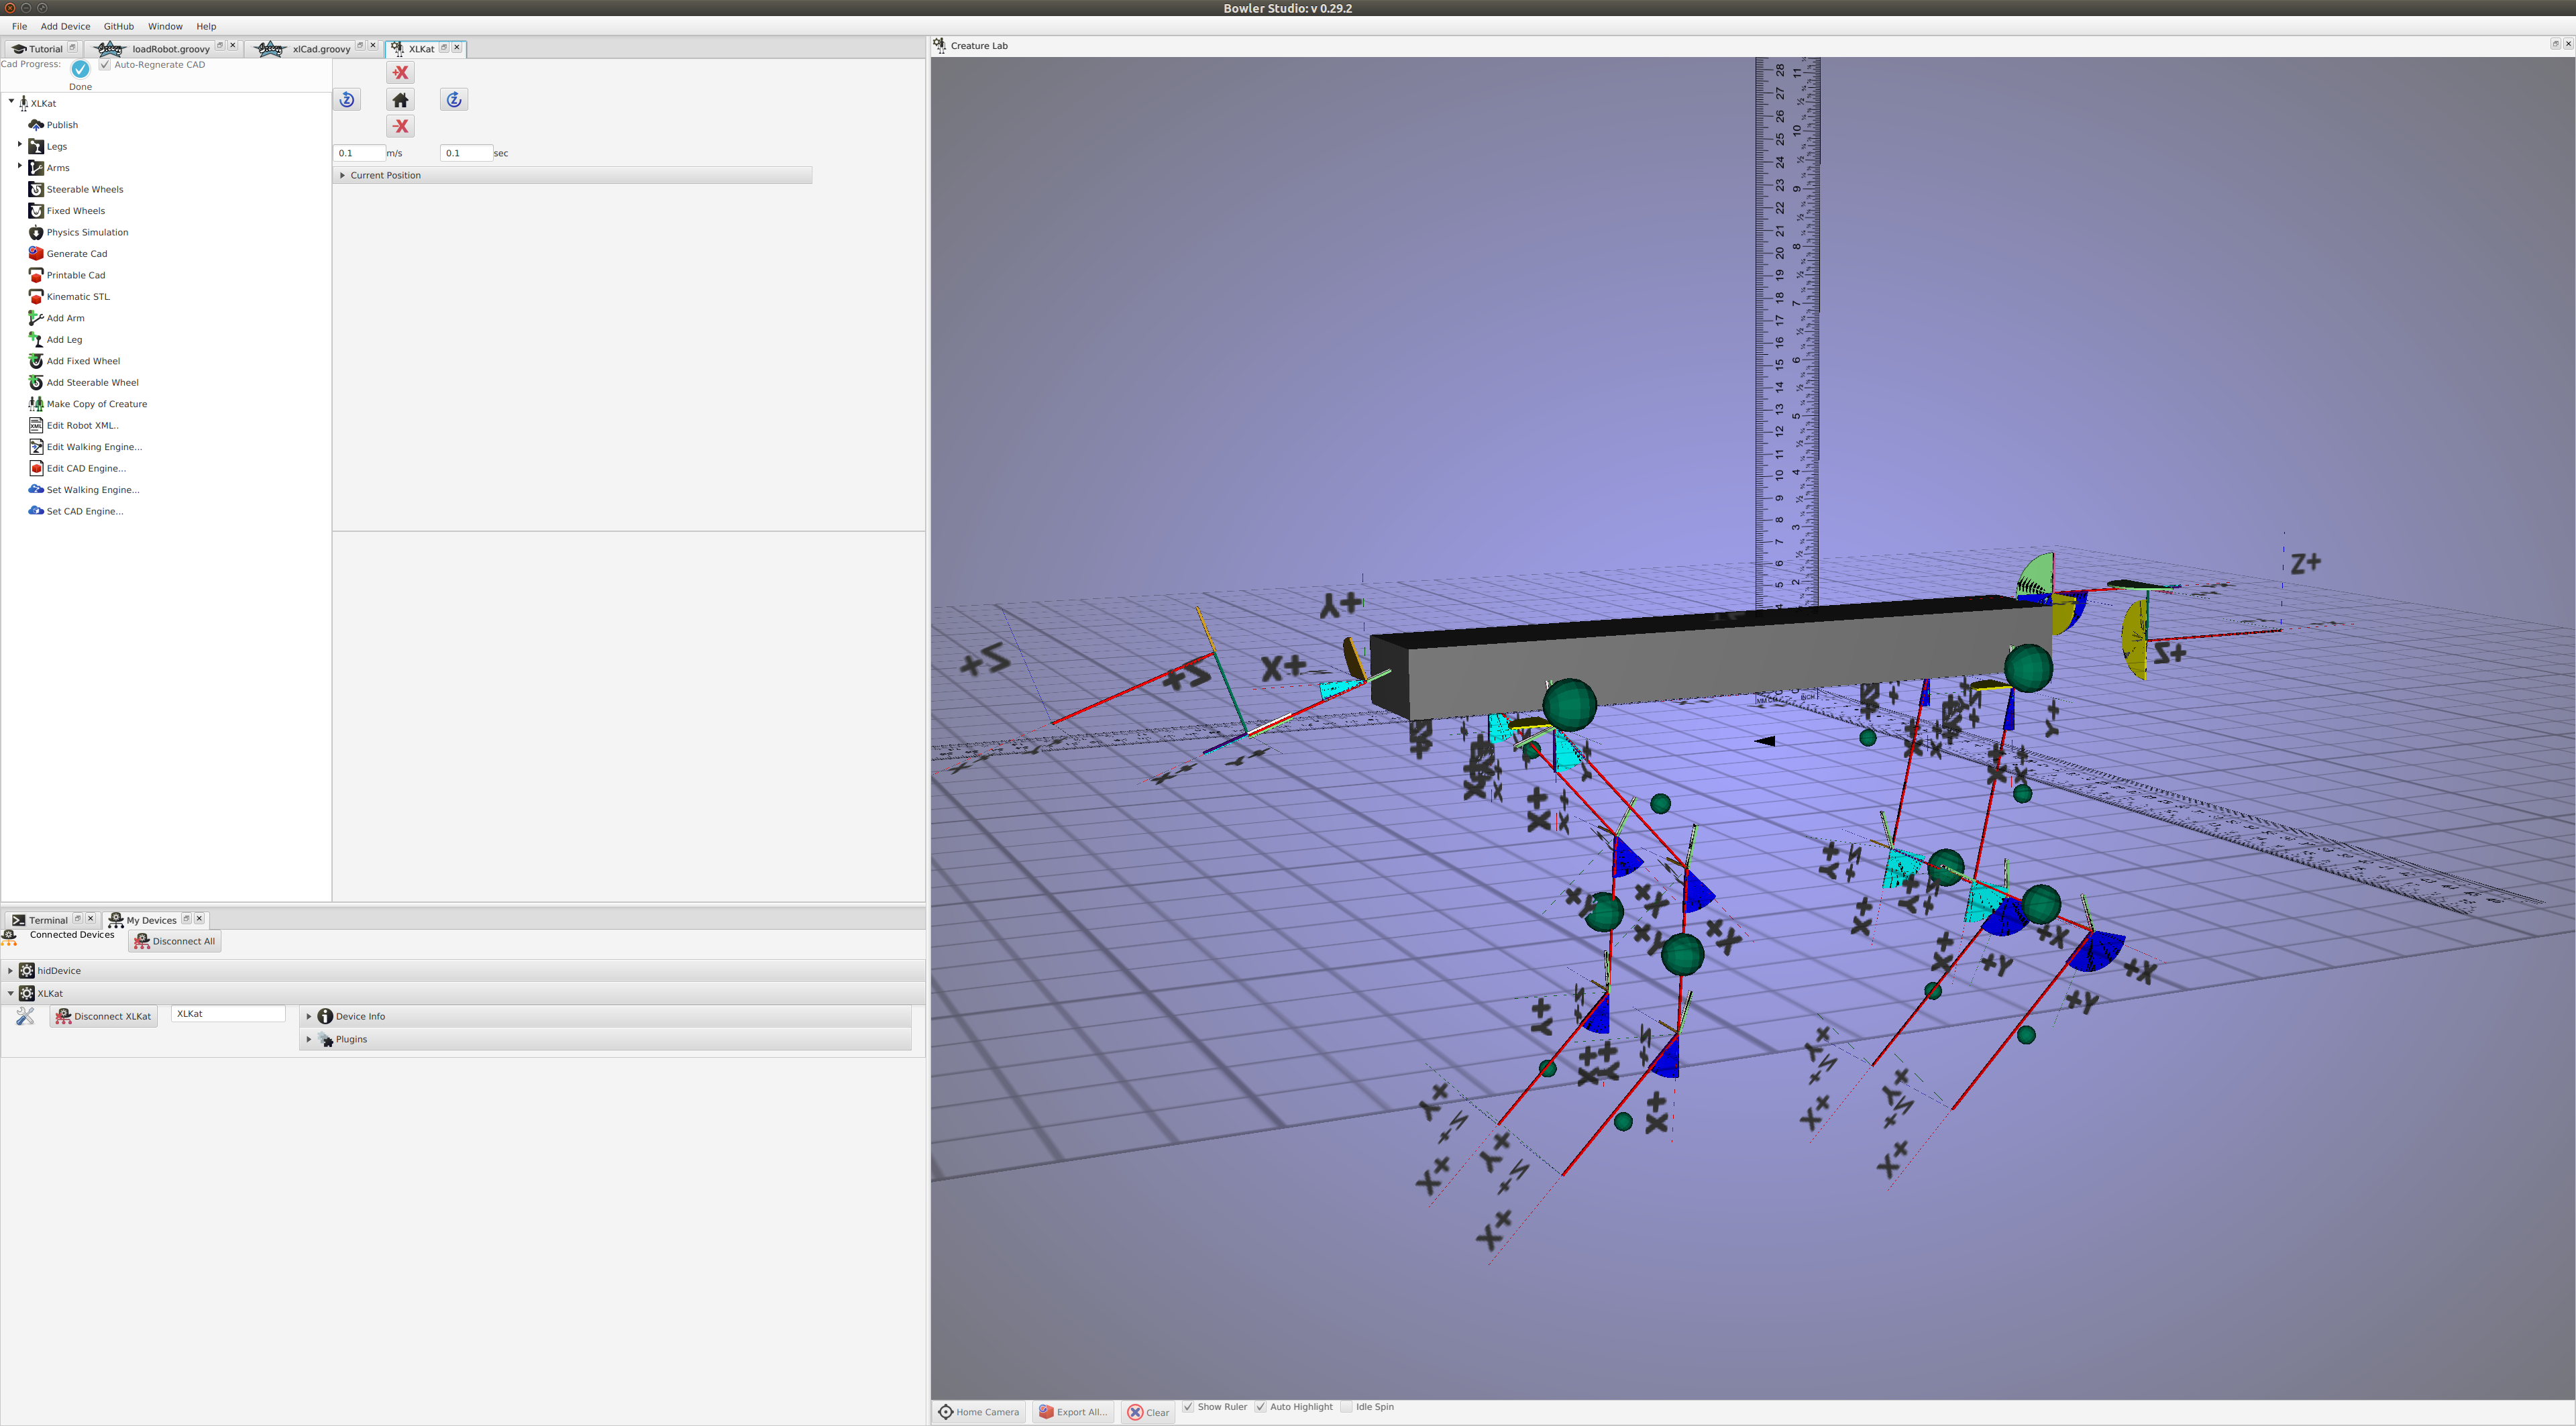
\includegraphics[width=0.5\textwidth]{figures/BowlerVis.png}
            \caption{The Implemented Visualization Tool}
            \label{fig:VisualizationTool}
        \end{figure}
        
        % Insert a description of the figure above
        We also added a flag that would allow us to switch between this tool and the full rendering of the robot for demonstration purposes.
    \subsubsection{High Level Controller: Odroid vs Raspberry Pi 3}
        Originally, we wanted to use an Odroid XU4, due to its floating point computation performance. However, when installing and running Bowler Kernel on the Odroid, we realized we needed the affines from the JavaFX library. There was no implementation of JavaFX on the Odroid's processor, and the attempt to install from source did not work. Therefore, we switched to the Raspberry Pi 3 B+, since JavaFX was compatible with it. Although performance was a concern, we were still able to stay under 1ms per cycle.
    \subsubsection{Our IHMC Implementation}
        IHMC's library set is a very powerful tool for walking robotics. It includes libraries for dynamic modeling, walking gaits, and simulation for development. The library set has successfully been used on robots including Boston Dynamics' ATLAS and NASA's Valkyrie Humanoid, and was very promising. However, documentation and support quickly became an issue, since the libraries were just beginning to be released and documentation had yet to be published. We did attempt to develop our software with this system, but it became clear that moving forward would become increasingly more difficult with less and less documentation. However, Figure \ref{fig:IHMCImplementation} shows our simulation environment we created to test our code.
        \begin{figure}
            \centering
           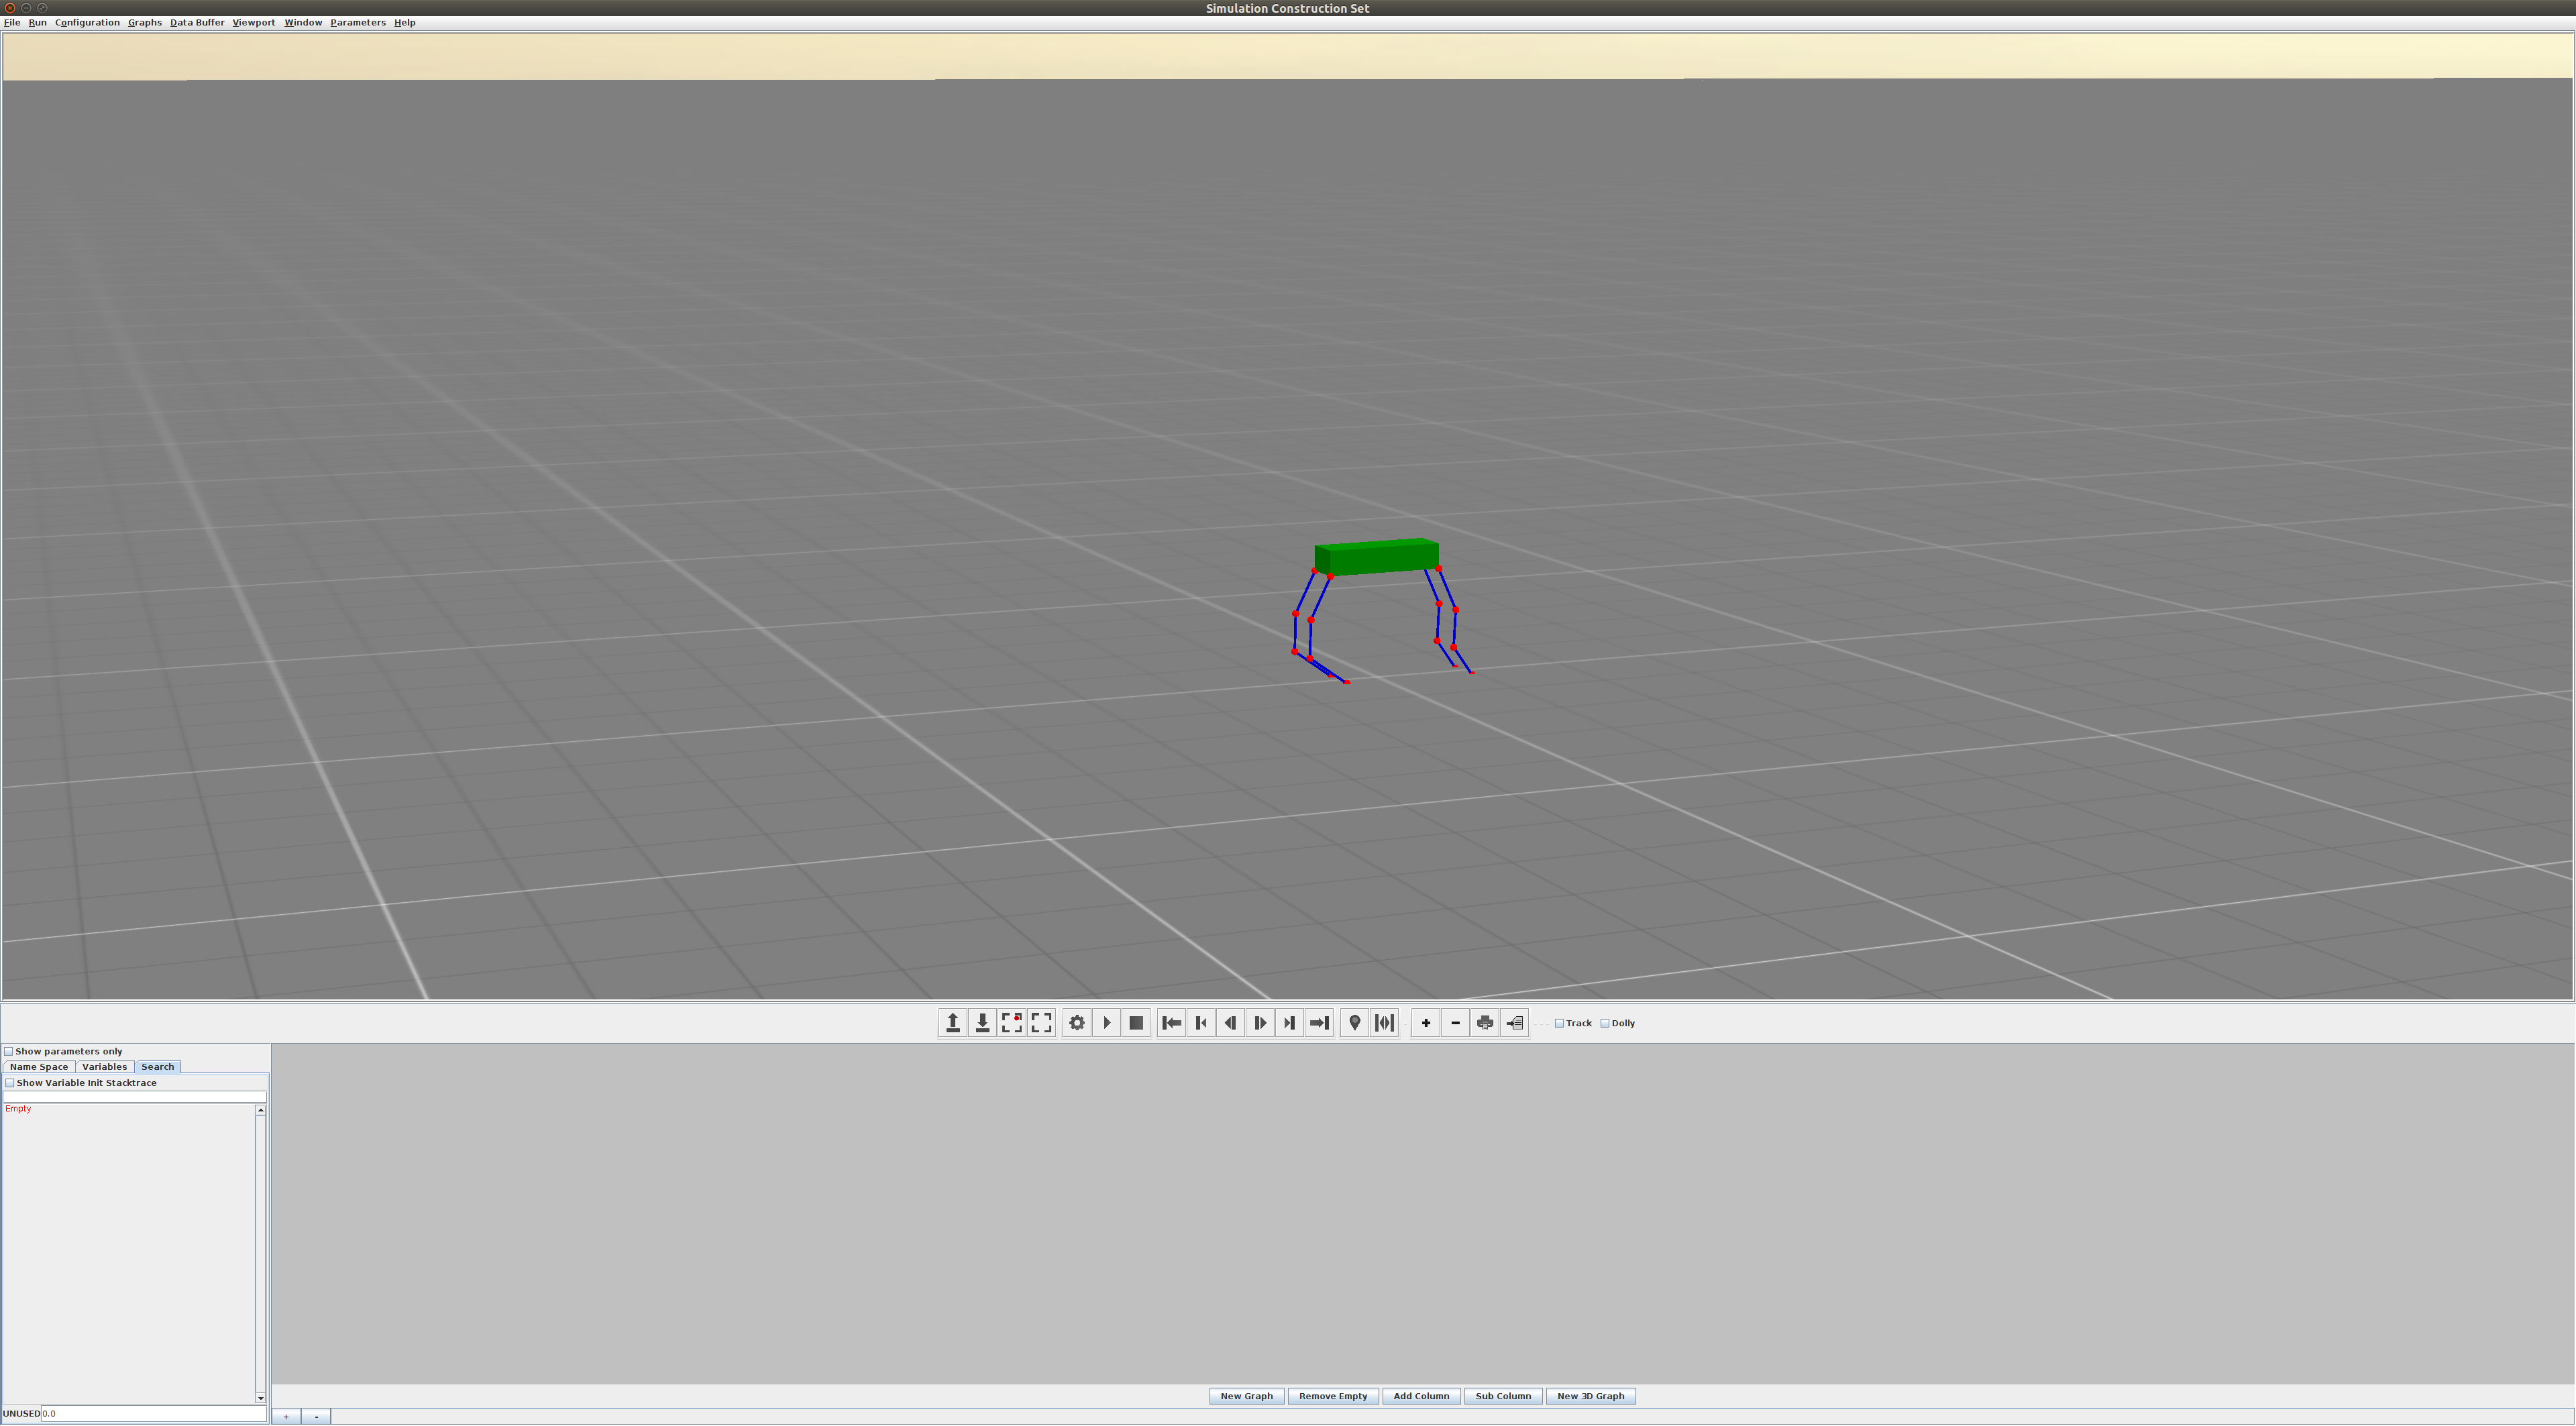
\includegraphics[width=0.5\textwidth]{figures/IHMCImplementation.png}
            \caption{Our IHMC Implementation}
            \label{fig:IHMCImplementation}
        \end{figure}